\documentclass[12pt]{article}

\usepackage{fullpage}
\usepackage{graphicx}
\usepackage{graphics}
\usepackage{mdwlist}
\usepackage{float}
\usepackage{caption}
\usepackage{wrapfig}
\usepackage{listings}
\usepackage{enumerate}
\usepackage{hyperref}
\usepackage{color}
\usepackage{longtable}

% christos: these look closer to NSF specs\dots
\setlength{\oddsidemargin}{0.0in}
\setlength{\evensidemargin}{0.0in}
\setlength{\textwidth}{6.5in}
\setlength{\headheight}{0.0in}
\setlength{\topmargin}{0.0in}
% \setlength{\textheight}{9.0in}
\setlength{\textheight}{9in}
\addtolength{\textheight}{-\topmargin}
\addtolength{\textheight}{-\headheight}
\addtolength{\textheight}{-\headsep}
\addtolength{\textheight}{-\footskip}

\definecolor{dkgreen}{rgb}{0,0.6,0}
\definecolor{gray}{rgb}{0.5,0.5,0.5}
\definecolor{mauve}{rgb}{0.58,0,0.82}

\lstset{frame=tb,
  language=SQL,
  aboveskip=3mm,
  belowskip=3mm,
  showstringspaces=false,
  columns=flexible,
  basicstyle={\small\ttfamily},
  numbers=none,
  numberstyle=\tiny\color{gray},
  keywordstyle=\color{blue},
  commentstyle=\color{dkgreen},
  stringstyle=\color{mauve},
  breaklines=true,
  breakatwhitespace=true,
  tabsize=3
}

\begin{document}

\newcommand{\beq}{\begin{equation}}
\newcommand{\eeq}{\end{equation}}
\newcommand{\bit}{\begin{itemize*}}
\newcommand{\eit}{\end{itemize*}}
\newcommand{\goal}[1]{ {\noindent {$\Rightarrow$} \em {#1} } }
\newcommand{\hide}[1]{}
\newcommand{\comment}[1]{ {\footnotesize {#1} } }
\newtheorem{lemma}{Lemma}
\newtheorem{theorem}{Theorem}
\newtheorem{proof}{Proof}
\newtheorem{defn}{Definition}
\newtheorem{algo}{Algorithm}
\newtheorem{observation}{Observation}

\setlength{\belowcaptionskip}{-20pt}
\setlength{\abovecaptionskip}{5pt}

\title{Graph Mining}


\author{ {\em Yuwei Zhang} \\
	    MCDS \\
	    CMU\\
	    {\tt yuweiz1@andrew.cmu.edu}
	 \and
	 {\em Silun Wang} \\
	     MCDS \\
	     CMU\\
	     {\tt silunw@andrew.cmu.edu}
}

\maketitle

\section{Introduction}
Many realworld datasets contain valueable information to be discovered. In this paper, we present a graph mining tool -- \textbf{Graph Miner} which employs simple SQL commands for efficiently mining large datasets through PostgresSQL. On 15 realworld datasets, we present our discoveries about global patterns and anomoly detections.

\section{Phase1: Survey}
    \label{sec:survey}
    
\subsection{Papers read by Yuwei Zhang }
\textbf{Evaluating cooperation in communities with k-core structure}
\cite{Evaluating}
\begin{itemize*}
\item {\em Problem Definition}: The paper focuses on community detection and evalutation, which means dense connections among some of the nodes. The author make some novel changes to the k-core concepts including updating mtric for evaluating cohesiveness, assigning weights on the edges and other extended experimental evaluation.
\item {\em Summary}:The original k-cores algorithm keeps deleting nodes whose degree are less than k and thus take the number of each set of vertices in the subgraph to do the evalution, which fails in the case where many co-authors have equal weight. This paper improves the method to define a co-authorship edge weight instead and recompute the evalution metrics with restrictions considered. In the expriment stage, testing on an unfiltered graph turns out to be extremely biased while on a filtered one(those co-author a lot) the results seem to be resonable. When weights graph method is applied, the extrem cases where k is too big are ignored and the algorithm gives better results. 
\item {\em Shortcomings}:There is no standard metrics to evaluate these algorithms/methods propsed in the paper. Also when we consider the graphs as social networks, where the relationship between two nodes are more than just co-author, for instance we have flollow, like, dislike, the weighted method should be furthur adjusted and it might be hard to derive the best weighting formula.
\end{itemize*}

\textbf{Vertexica: your relational friends for graph analytics}
\cite{vertexica}
\begin{itemize*}
\item {\em Problem Definition}: To build a graph analysis tool, Vertexica, on top of a rdb that supports vertex-centric query interface. The system leverage the realational features and enable better graph analysis.
\item {\em Summary}:Vertexica supports user-friendly and high-performance graph analysis by injecting data storage, query processing and query interfaces and supports various kinds of relational database. The system consists of four main components: physical storage to store data, coordinator as the center management driver, worker as the conntainer for the computation programs and vertex computation to process user queries. Vertexica also take several optimization techniques including: table union instead of table join, paralleling workers to work on multicores or multi machines, vertex batching to partition the table and create new tables other than update the orgin information to boost the performance. The paper also includes some use case demonstrations. 
\item {\em Shortcomings}:Hand-coded sql implementations give even better performance in the experiments of the paper. Is it possibel to furthur optimize the performance when using the user-friendly vertex-centric query interface?
\end{itemize*}

\textbf{Visual Exploaration of Collaboration Networks based on Graph Degeneracy}
\cite{visual}
\begin{itemize*}
\item {\em Problem Definition}:To build a system that supports visual exploration of collaboration networks based on ranking of the nodes and filtering methods on the edges. It works on DBLP and is suitable for the large-scale networks.
\item {\em Summary}:The idea of graph degeneracy is derived from the conceptsof k-cores, which is introduced in previous paper(the one just summarized). Basically in this system, it extracts the co-authorship graph using the algorithm described in the other paper using filtered weighted egde algorithm, and then partition the graph to f-cores based on the Trim process. Then comes the ranking, by repeatedly performing the Trim procedure to remove more vertexes and in the end stores in the relation databse for furthur query. The system can be useful to demonstrate bibliographic data.
\item {\em Shortcomings}:For huge graphs, the k-core process may be extremly time-consuming. And it will take a long time for the system to reflect the updates in the graph.
\end{itemize*}


\subsection{Papers read by Silun Wang}
The first paper was the Belief Propogation paper by Wolfgang Gatterbauer, Stephan Gunnemann, Danai Koutra, and Christos Faloutsos
\cite{BeliefPro}
\begin{itemize*}
\item {\em Problem Definition}: In big social networks, sometimes we need to infer the labels for particular nodes via transductive inference or semi-supervised learning. The classical belief propagation algorithm is widely used in such scenario, but it does not guarantee convergence in loopy graphs. In this paper, the authors propose Linearized Belief propagation and Single-pass belief propagation which are based on different restrictions and assumptions and much faster than BP.
\item {\em Summary}:
    In a nutshell, LBP and SBP have the following advantages over BS:
    \begin{enumerate}
	\item Have convergence guarantees
	\item Have closed-form solutions, thus reducing computational cost
	\item Can be implemented on standardized SQL
	\item SBP can be updated incrementally
	\end{enumerate}
	LBP requires messages are normalized, thus the final belief matrix can be calculated via elegant matrix operations. SBP is based on the assumption that the impact of inference damps with length of paths. To obtain the final belief matrix, each node and each edge only need to be visited once.
\item {\em Shortcomings}:
      The Daubechies wavelets require a wrap-around setting,
      which may lead to non-intuitive results.
\end{itemize*}

The second paper was the k-core decomposition paper by Ignacio Alvarez-Hamelin, Luca Dall’Asta, Alain Barrat, and Alessandro
\cite{kcore}
\begin{itemize*}
\item {\em Problem Definition}: To visualize large complex networks is a big challenge, especially when you want clarity of graph and maintaining as much information as possible in the meantime. In this paper, the authors present an effective algorithm — k-core decomposition to visualize large complex networks in 2D dimension.
\item {\em Summary}:
K-core decomposition introduces several terms: coreness, shell, cluster. It assigns each vertex a polar coordinate, thus visualizing a large complex network in 2D dimension while preserving relative hierarchical structures, connectivity and clustering properties, as well as interrelationship between hierarchies. What’s more, the overall time complexity is only linear as $O(n + e)$.
\item{\em Shortcomings}:
In order to obtain a readable layout, we need to tune several parameters. Can we learn these parameters automatically? Also, for huge networks, even a k-core decomposed graph seems to be nasty. Future work might need to combine nodes into a cluster and visualize a cluster via a simplified motif representation.
\end{itemize*}

The third paper was the visualization paper by Cody Dunne and Ben Shneiderman
\cite{motif}
\begin{itemize*}
\item{\em Problem Definition}:
Big data explosion results in huge and complex networks. In order to understand the relationship between entities and also individual attributes, traditional statistical charts are not applicable. Node-link diagrams are introduced and quickly excels among others. However, some node-link diagrams require relatively large screen space while containing little or repeated information, and optimization for the layout is NP hard. We need a more simplified visualization method which preserves important information.
\item{\em Summary}:
Authors of this paper on one hand defines three kinds of motifs: fan, connector and clique. A fan consists of a head node connected to leaf nodes with no other neighbors. A connector motif consists of functionally equivalent span nodes that solely link a set of anchor nodes. A clique motif consists of a set of member nodes in which each pair is connected by at least one link. On the other hand, the author presents an effective algorithm for motif detection with polynomial time complexity. For example, they use the obvious algorithm for detecting fan motifs which has a run time complexity of O($|G.nodes|$*average neighbor count) and in order to find all cliques they use the Tomita algorithm. After replacing the motifs with more representative glyphs, the graph requires much less screen space and layout effort. It helps us more easily understand the network and even discover some hidden relationships. 
\item{\em Shortcomings}:
Users need to be trained for a short time to fully understand this new representation. It is ambiguous in choosing clique motifs because they often overlap with each other. Future work could present users with these overlaps and relative confidence on different partitions.
\end{itemize*}



\section{Phase1: Unit Tests}
    \label{sec:experiments}
    \subsection{Test Case I}

\begin{figure}[H]
\minipage{0.58\textwidth}
  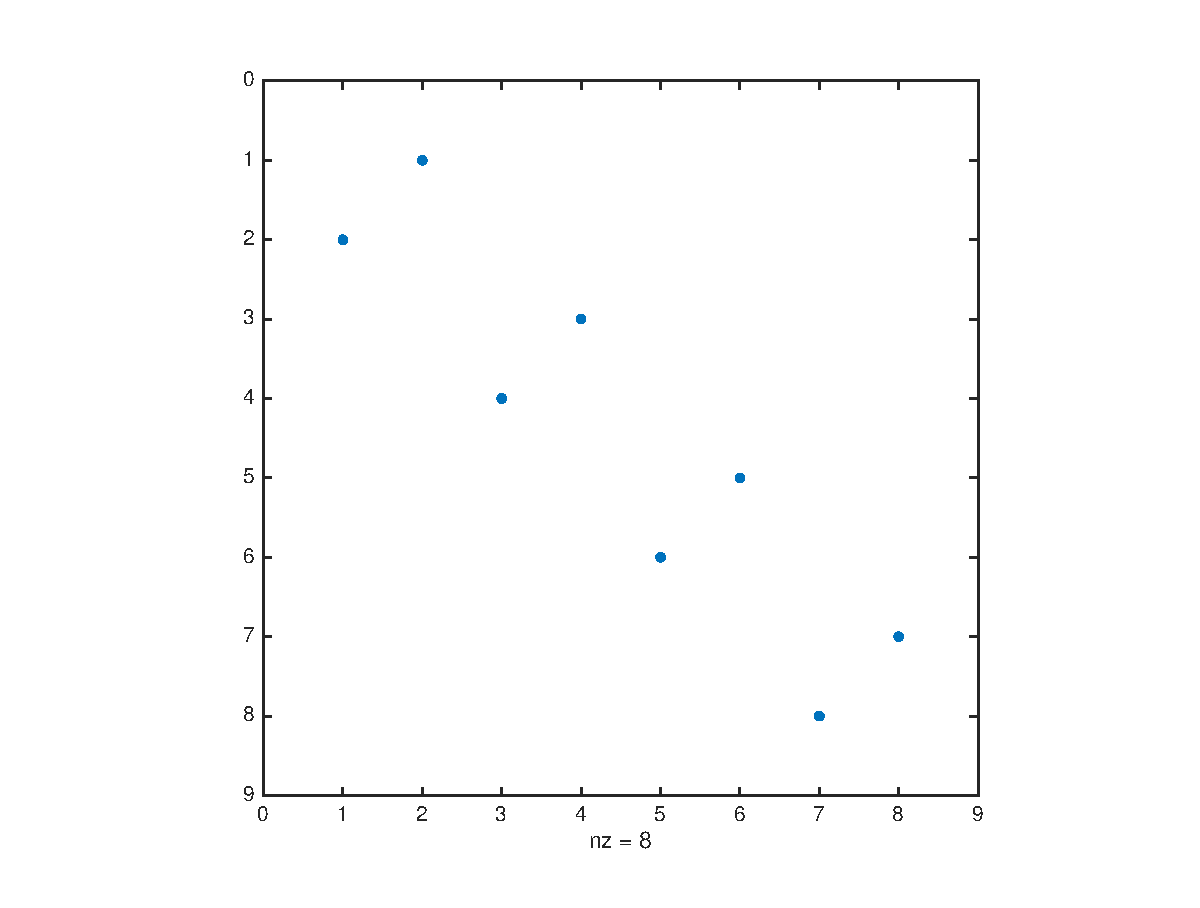
\includegraphics[width=\linewidth]{spy1.eps}
  \caption{Adjacency Matrix}
\endminipage\hfill
\minipage{0.38\textwidth}
  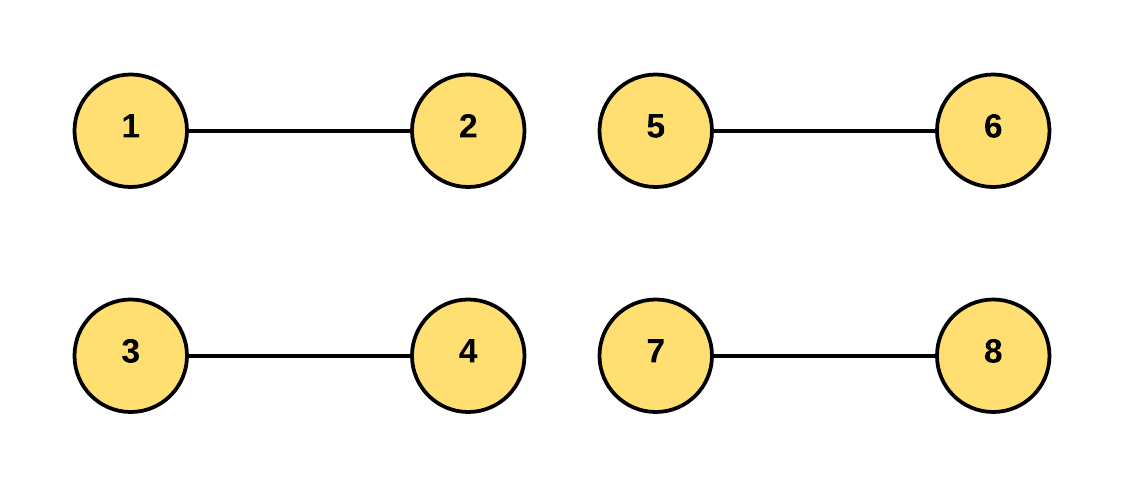
\includegraphics[width=\linewidth]{graph1}
  \caption{Graph}
\endminipage
\end{figure}
\begin{verbatim}
k core value:
[(1, 1), (2, 1), (3, 1), (4, 1), (5, 1), (6, 1), (7, 1), (8, 1)]

Degree distribution:
1 --> 8

Number of connected components: 4
\end{verbatim}

\subsection{Test Case II}

\begin{figure}[H]
\minipage{0.58\textwidth}
  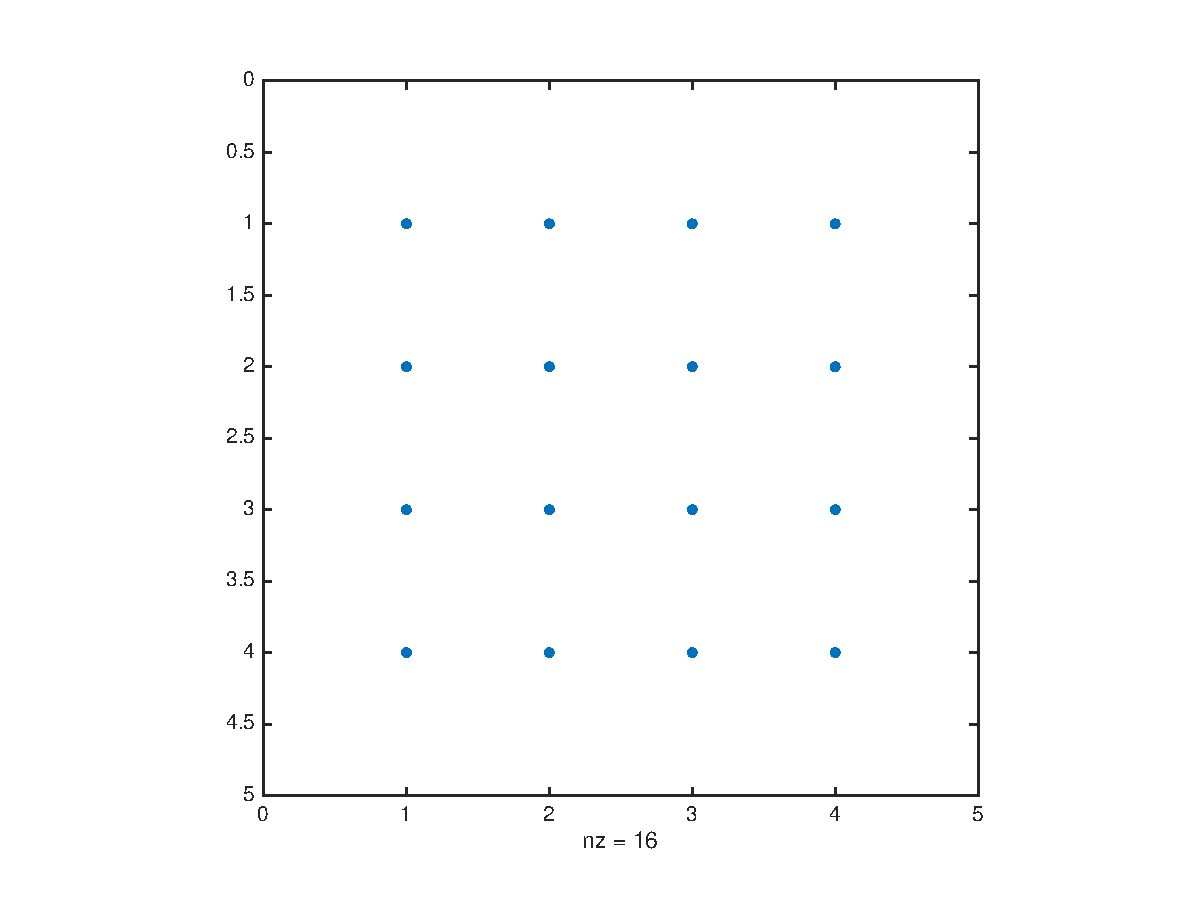
\includegraphics[width=\linewidth]{spy2.eps}
  \caption{Adjacency Matrix}
\endminipage\hfill
\minipage{0.28\textwidth}
  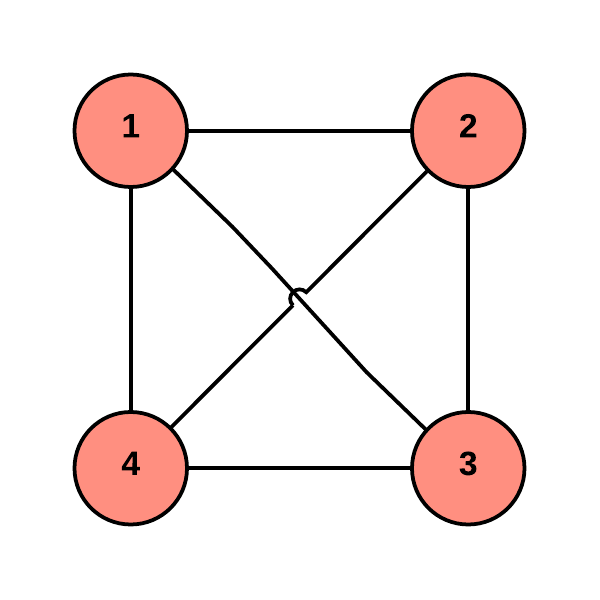
\includegraphics[width=\linewidth]{graph2}
  \caption{Graph}
\endminipage
\end{figure}
\begin{verbatim}
k core value:
[(1, 3), (2, 3), (3, 3), (4, 3)]

Degree distribution:
3 --> 4

Number of connected components: 1
\end{verbatim}

\subsection{Test Case III}
\begin{figure}[H]
\minipage{0.58\textwidth}
  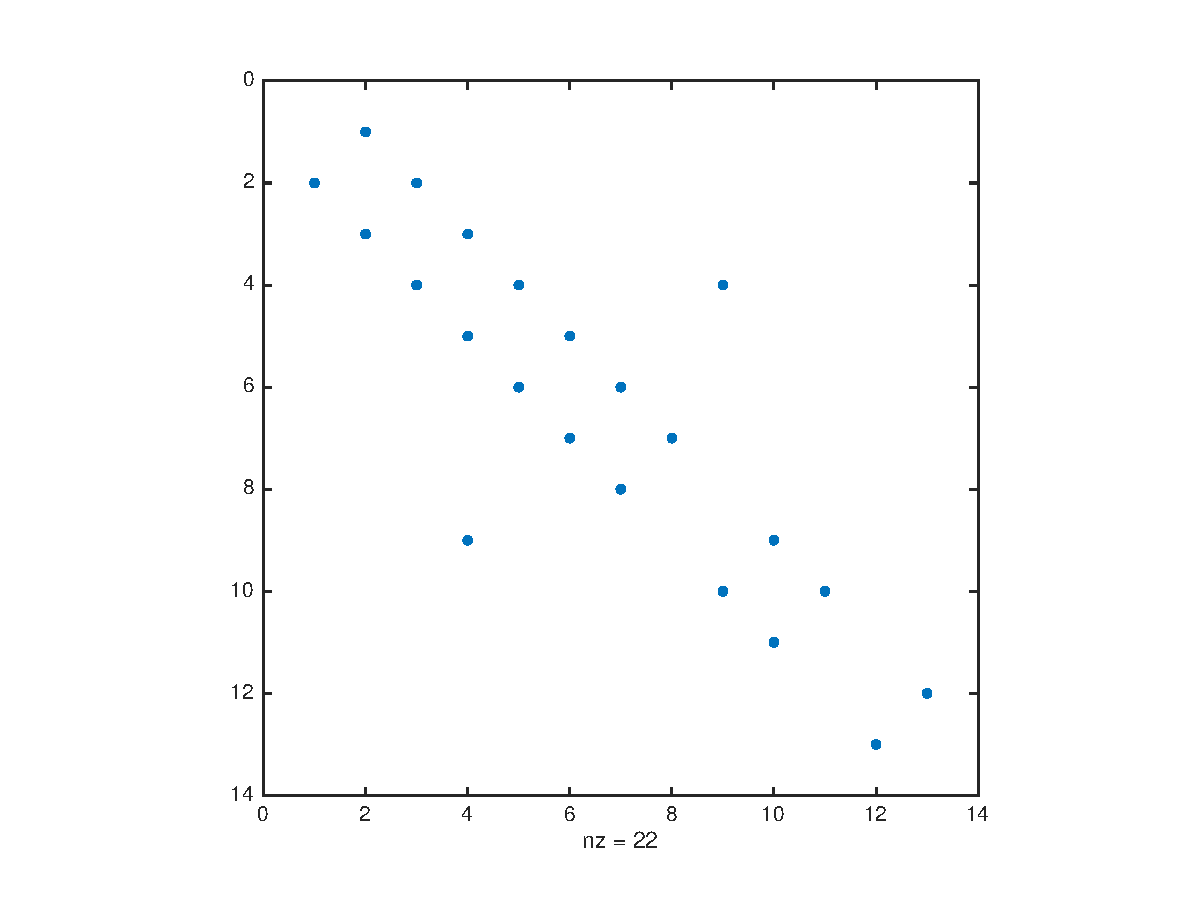
\includegraphics[width=\linewidth]{spy3.eps}
  \caption{Adjacency Matrix}
\endminipage\hfill
\minipage{0.38\textwidth}
  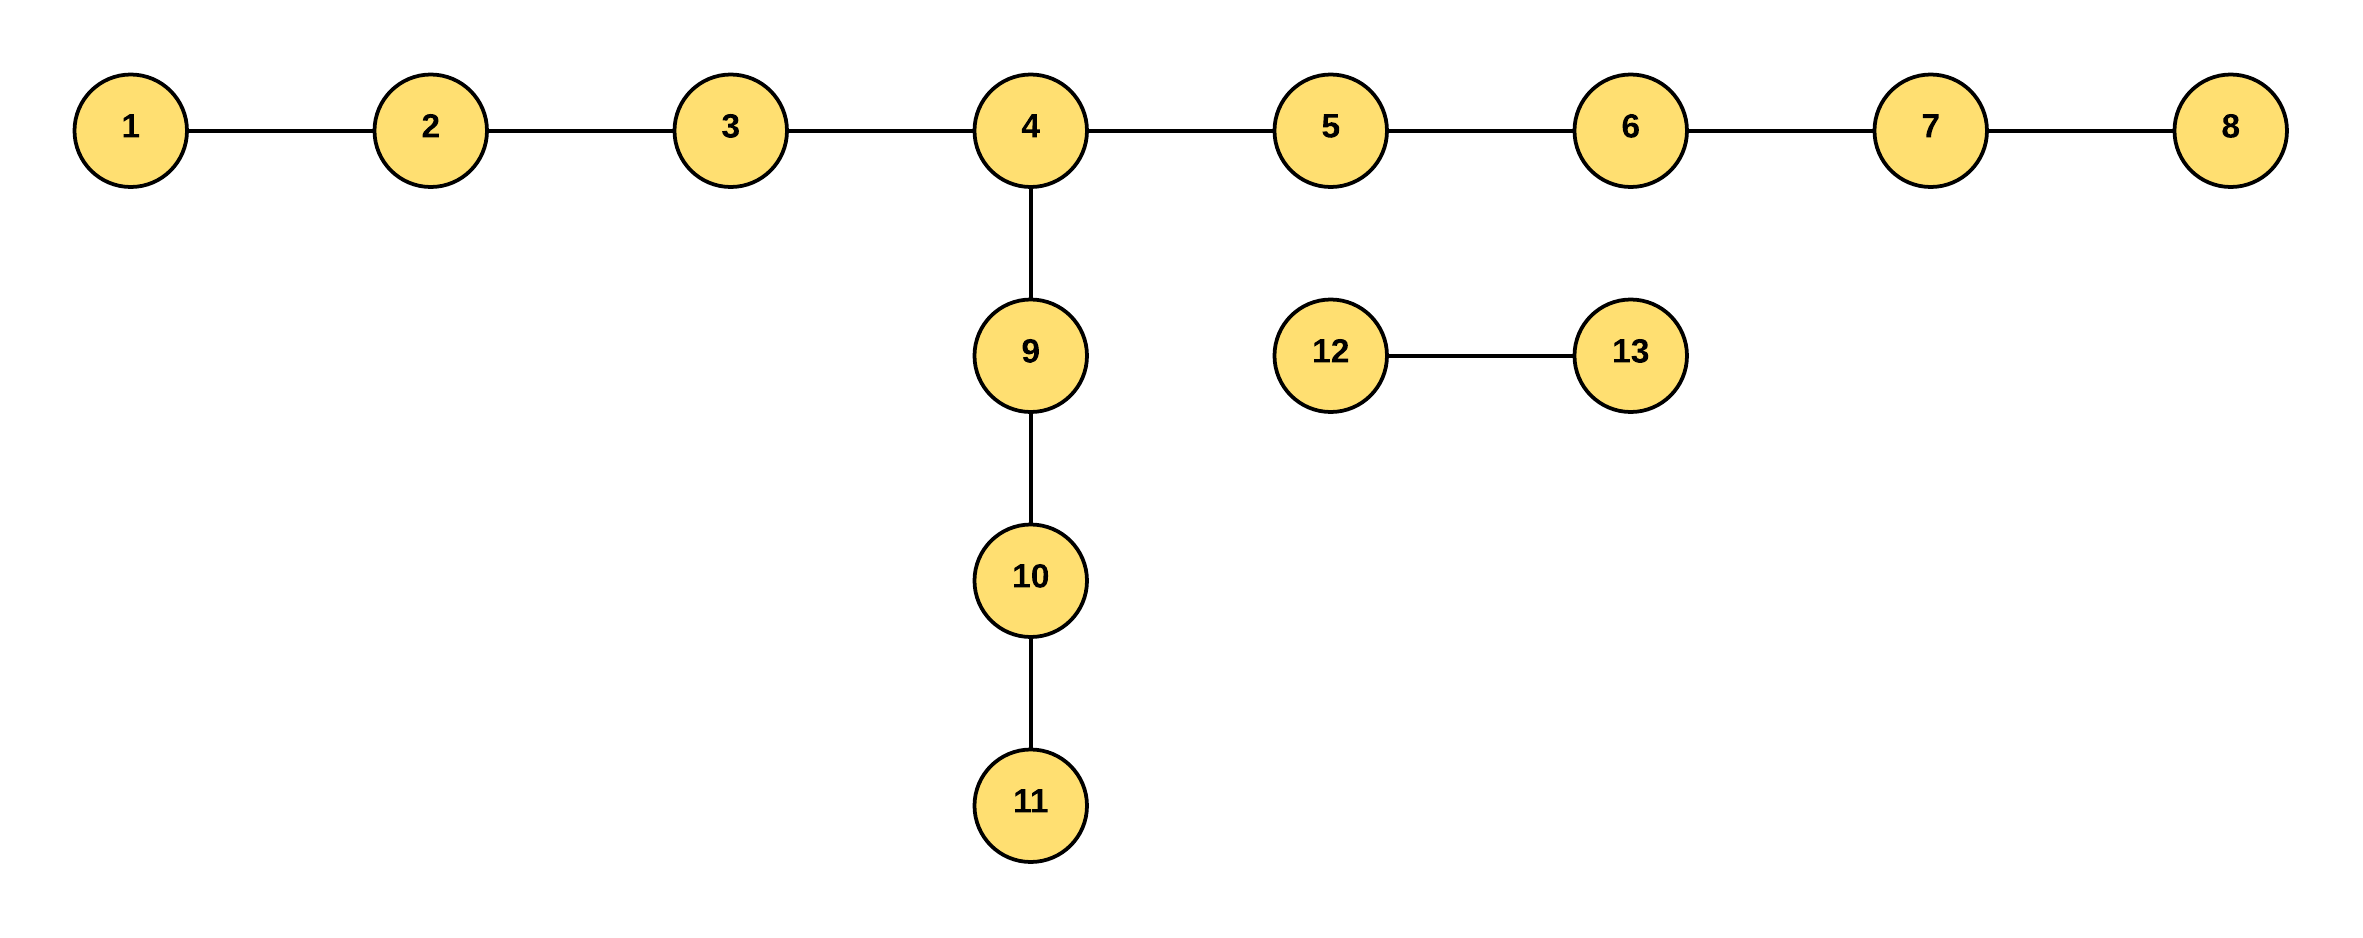
\includegraphics[width=\linewidth]{graph3}
  \caption{Graph}
\endminipage
\end{figure}

\begin{verbatim}
k core value:
[(1, 1), (8, 1), (11, 1), (12, 1), (13, 1), (2, 1), (7, 1), 
	(10, 1), (3, 1), (6, 1), (9, 1), (5, 1), (4, 1)]

Degree distribution:
1 --> 5
2 --> 7
3 --> 1

Number of connected components: 2
\end{verbatim}

\subsection{Test Case IV}
\begin{figure}[H]
\minipage{0.58\textwidth}
  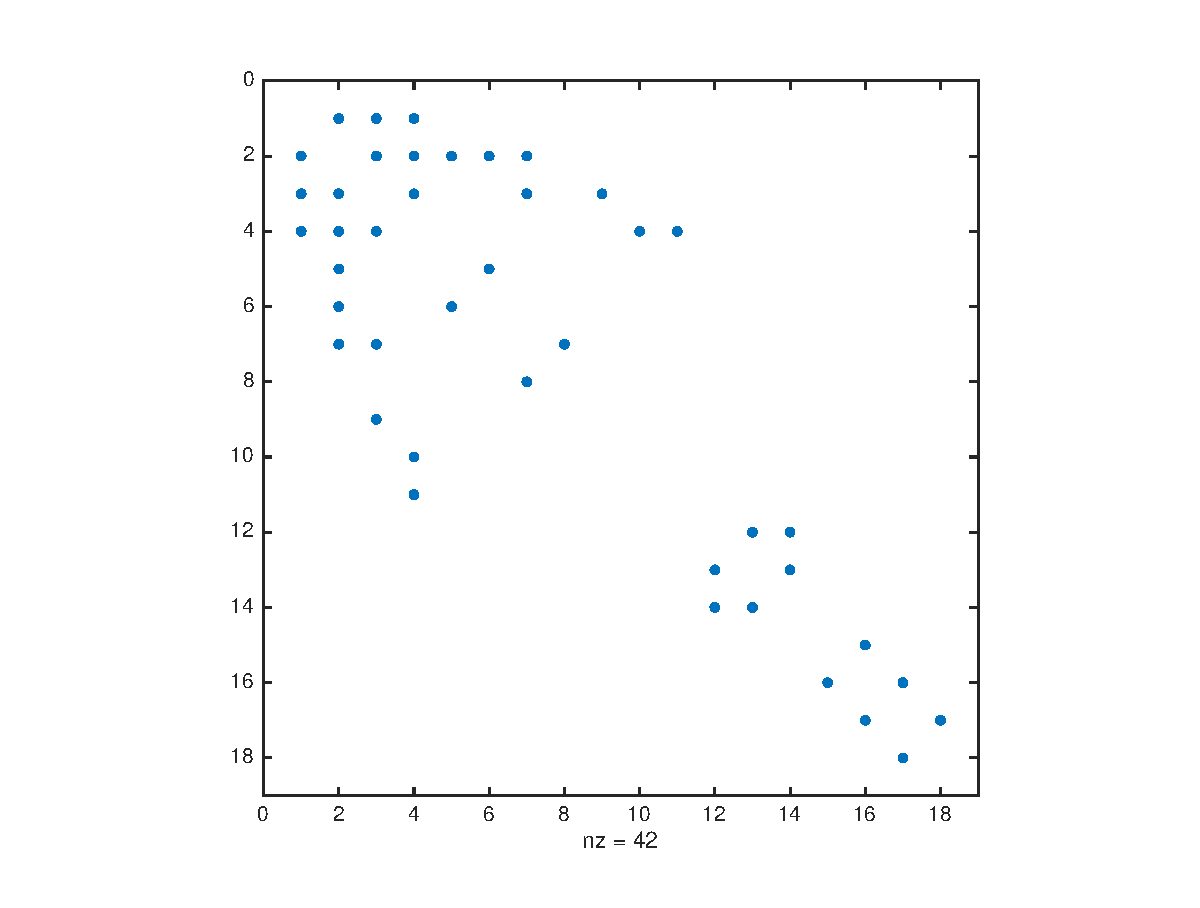
\includegraphics[width=\linewidth]{spy4.eps}
  \caption{Adjacency Matrix}
\endminipage\hfill
\minipage{0.38\textwidth}
  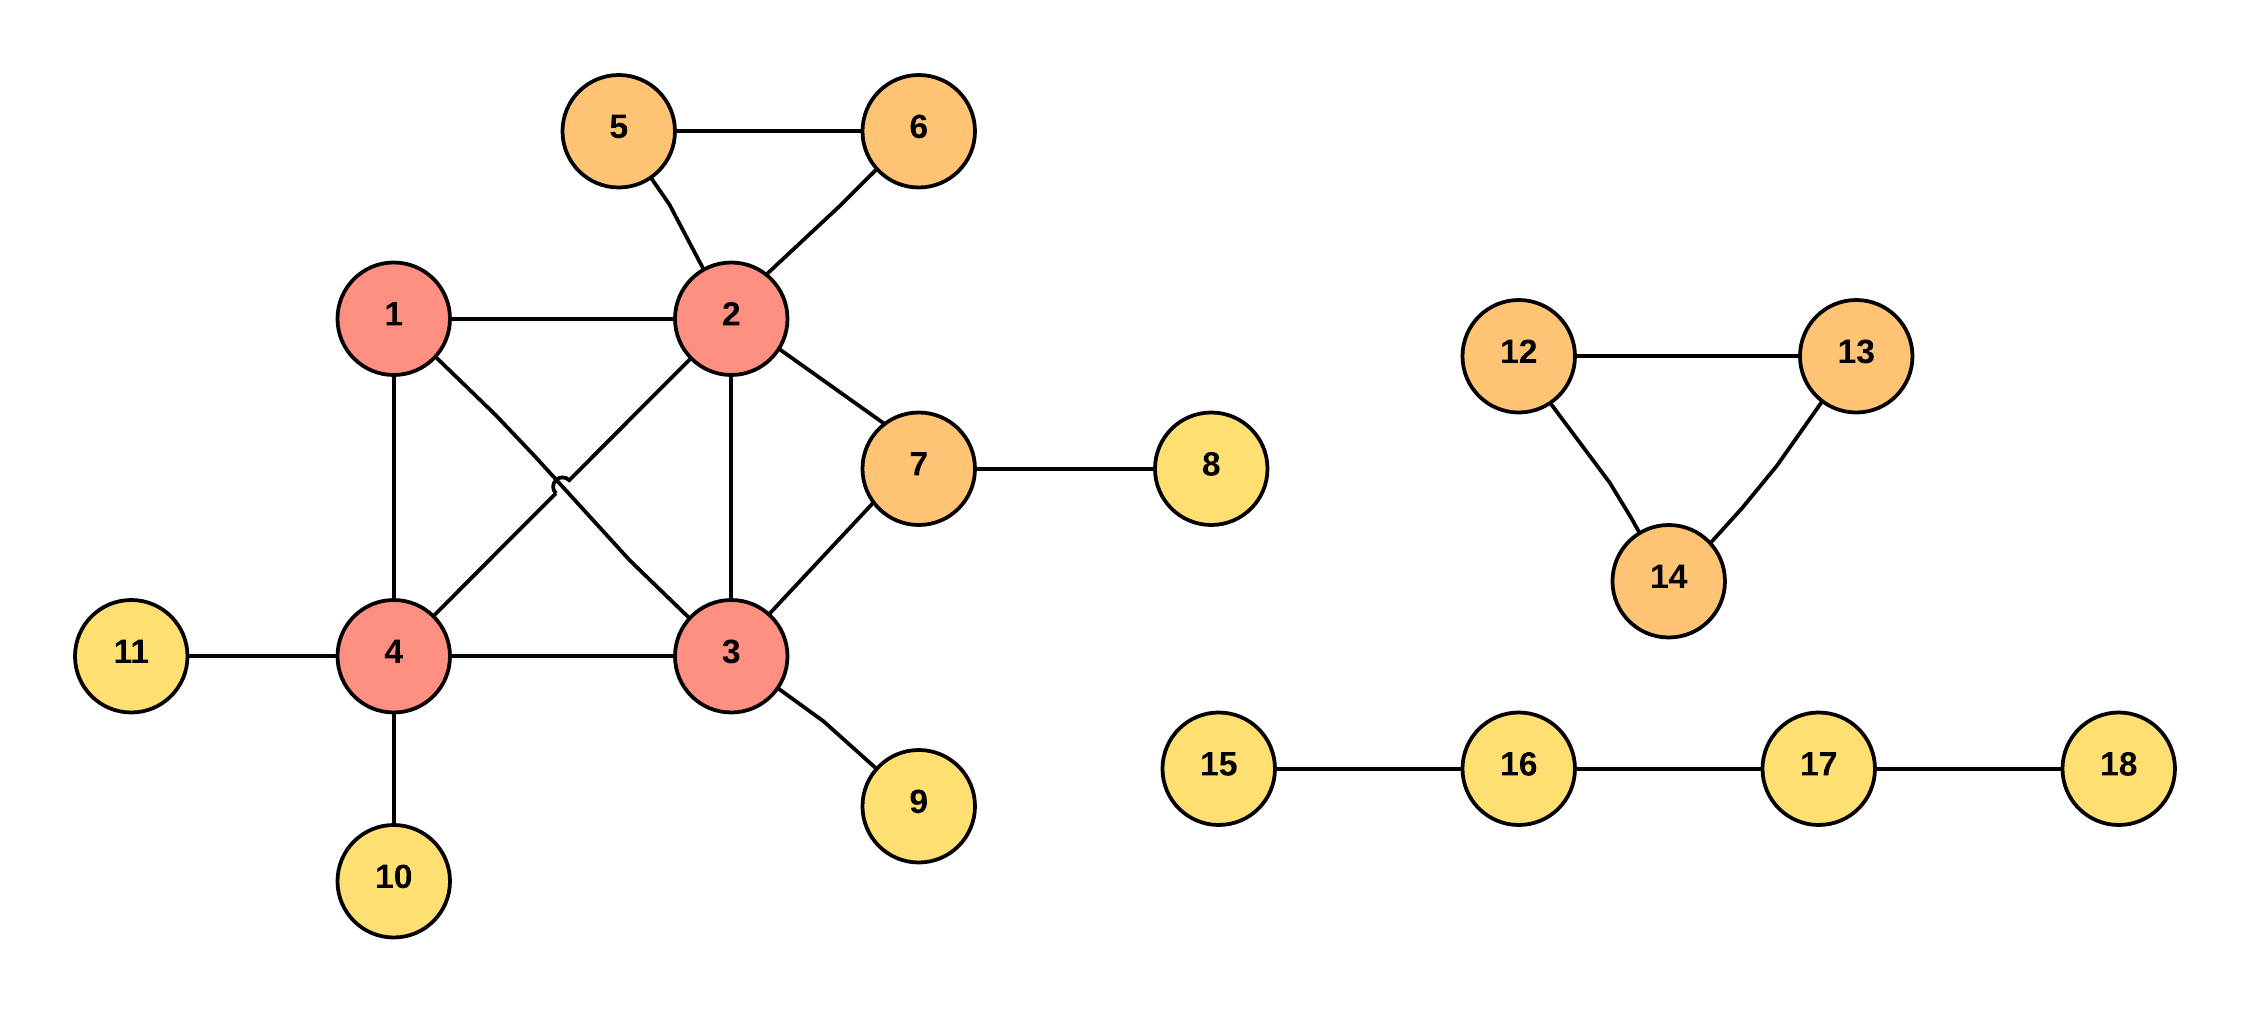
\includegraphics[width=\linewidth]{graph4}
  \caption{Graph}
\endminipage
\end{figure}

\begin{verbatim}
k core value:
[(8, 1), (9, 1), (10, 1), (11, 1), (15, 1), (16, 1), (17, 1), (5, 2), 
	(6, 2), (12, 2), (13, 2), (14, 2), (7, 2), (4, 3), (1, 3), (2, 3), (3, 3)]

Degree distribution:
1 --> 6
2 --> 7
3 --> 2
5 --> 2
6 --> 1

Number of connected components: 3
\end{verbatim}

\subsection{Test Case V}
\begin{figure}[H]
\minipage{0.58\textwidth}
  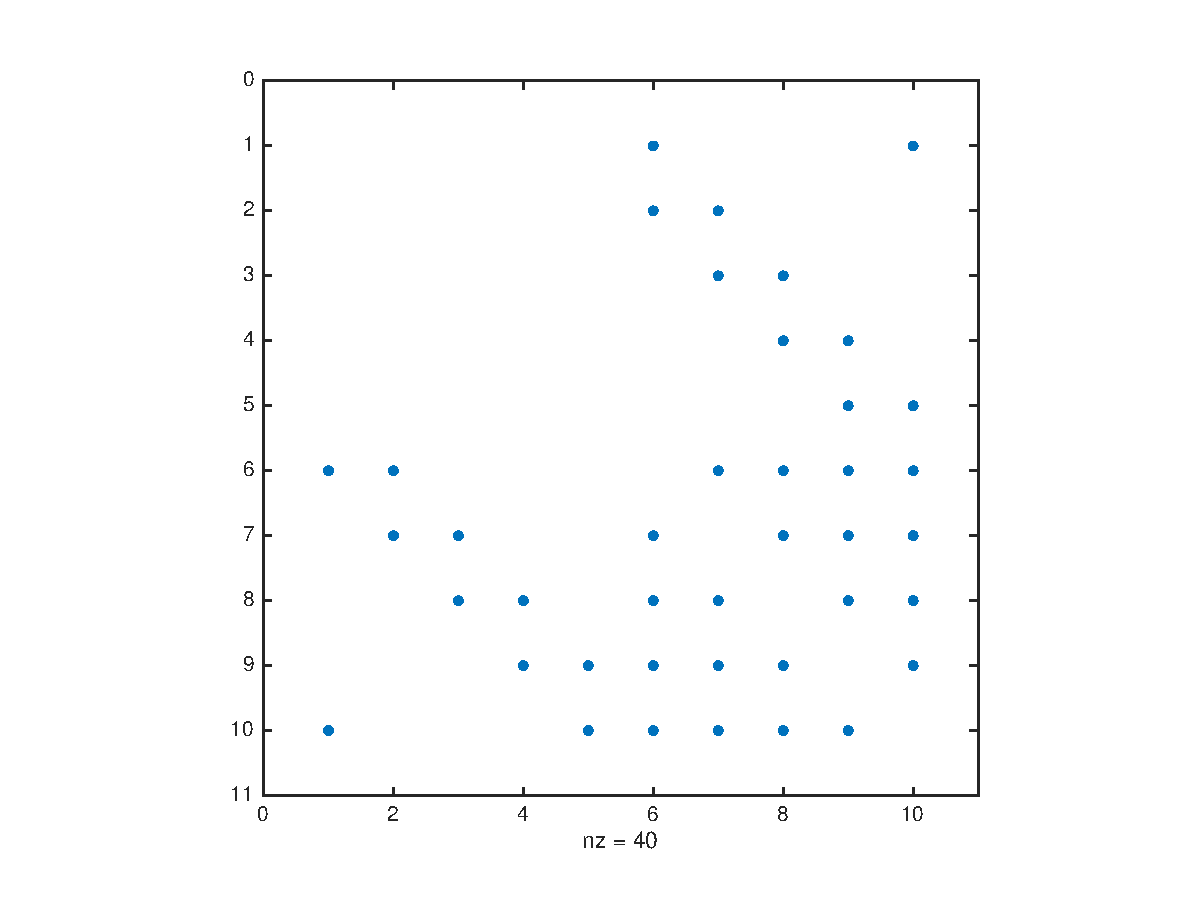
\includegraphics[width=\linewidth]{spy5.eps}
  \caption{Adjacency Matrix}
\endminipage\hfill
\minipage{0.38\textwidth}
  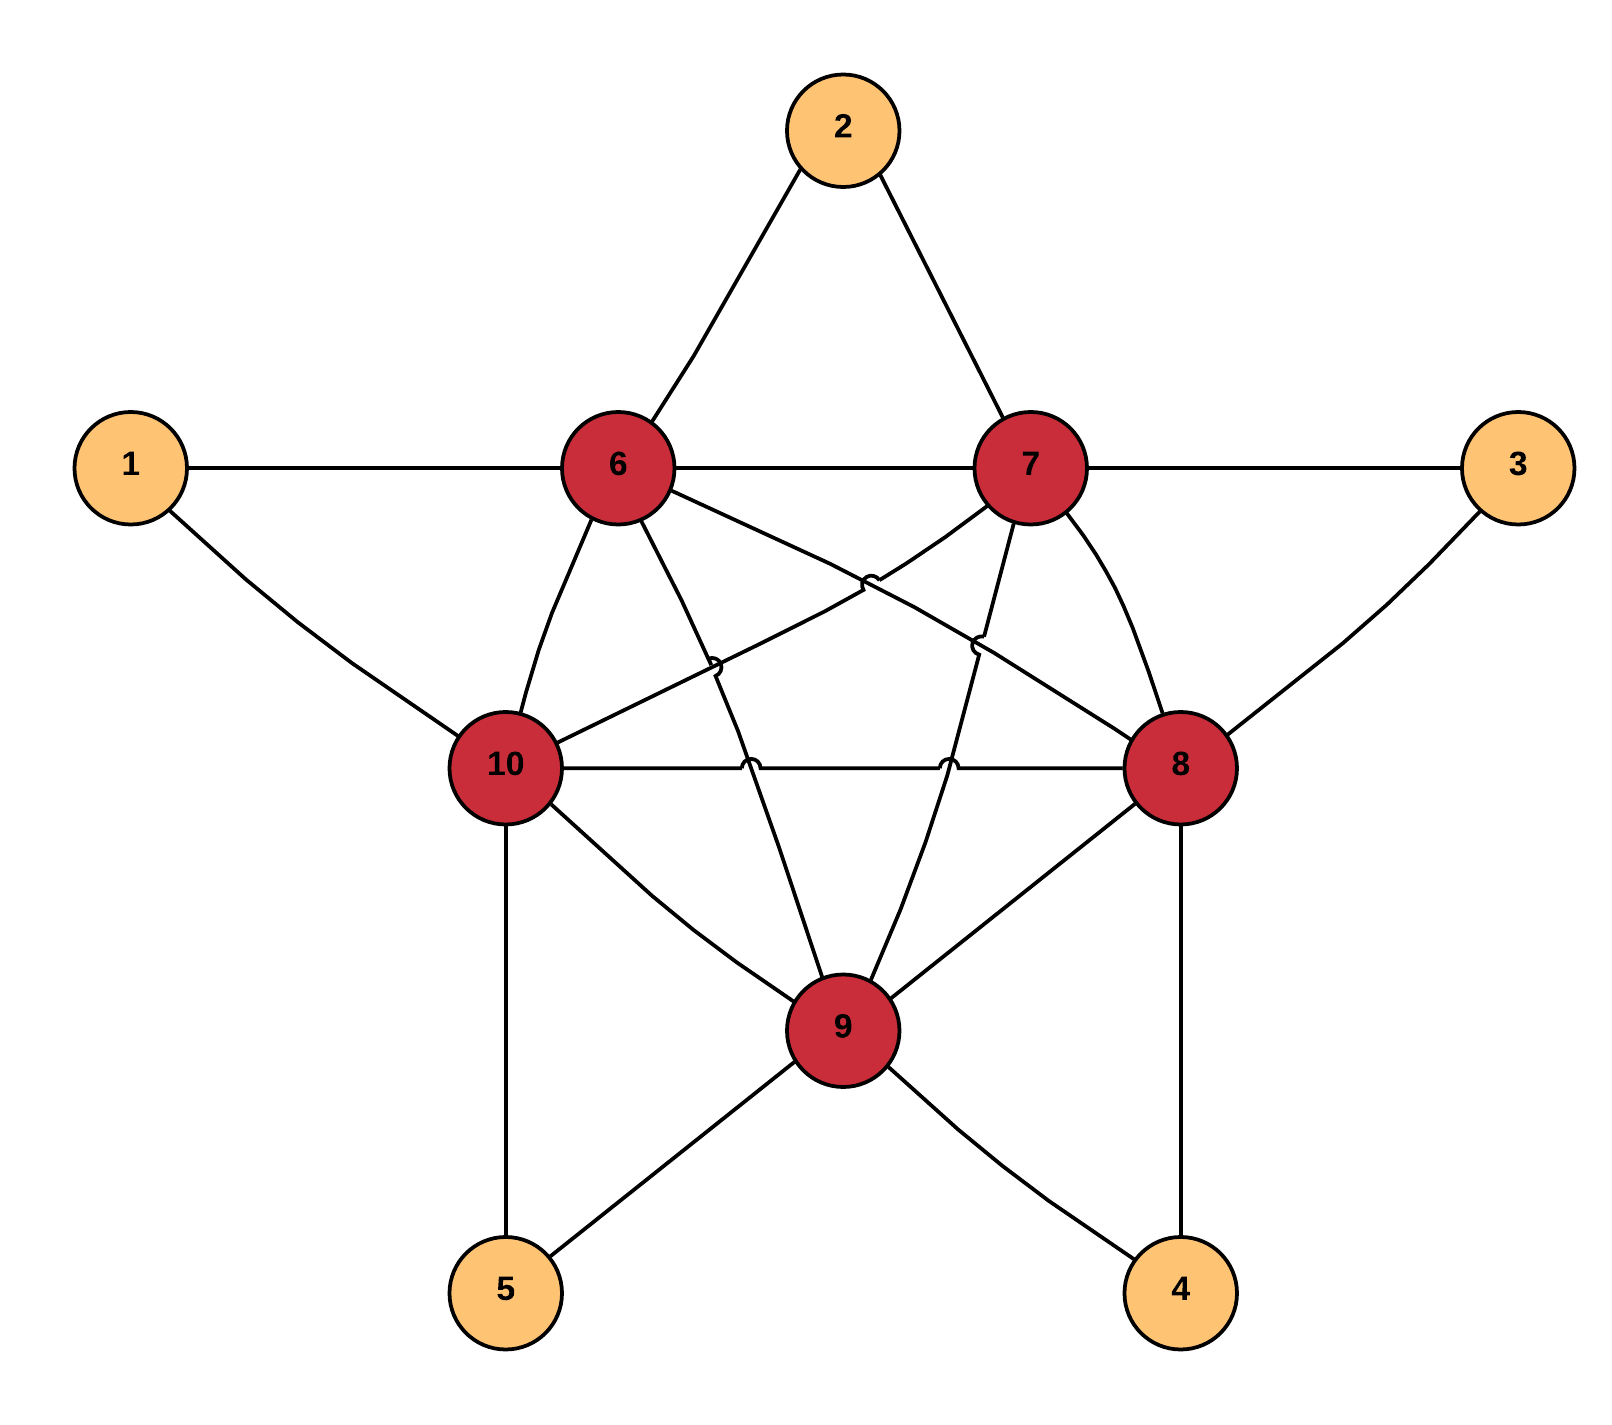
\includegraphics[width=\linewidth]{graph5}
  \caption{Graph}
\endminipage
\end{figure}

\begin{verbatim}
k core value:
[(2, 2), (3, 2), (4, 2), (5, 2), (1, 2), (7, 4), (6, 4), (8, 4), (9, 4), (10, 4)]

Degree distribution:
2 --> 5
6 -- > 5

Number of connected components: 1
\end{verbatim}

\section{Phase1: Experiment Results}
    \label{sec:conclusions}
    \subsection{Core value}
\begin{table}[!ht]
	\begin{tabular}{| l | l | l | l | l | l |}
	  \hline			
	  dataset & id = 0 & id = 17 & id = 9422 & id = 18475 & id = 27763 \\ \hline
	  soc-Slashdot0811 & 43 & 43 & 43 & 43 & 15\\ \hline
	  soc-Epinions1 & 67 & 43 & 2 & 10 & 4 \\
	  \hline  
	\end{tabular}
	\label{tab:a}
\end{table}

\subsection{Degeneracy value}
soc-Slashdot0811 : 55\\
soc-Epinions1 : 67\\


\subsection{Core value distribution}
\begin{figure}[H]
\minipage{0.48\textwidth}
  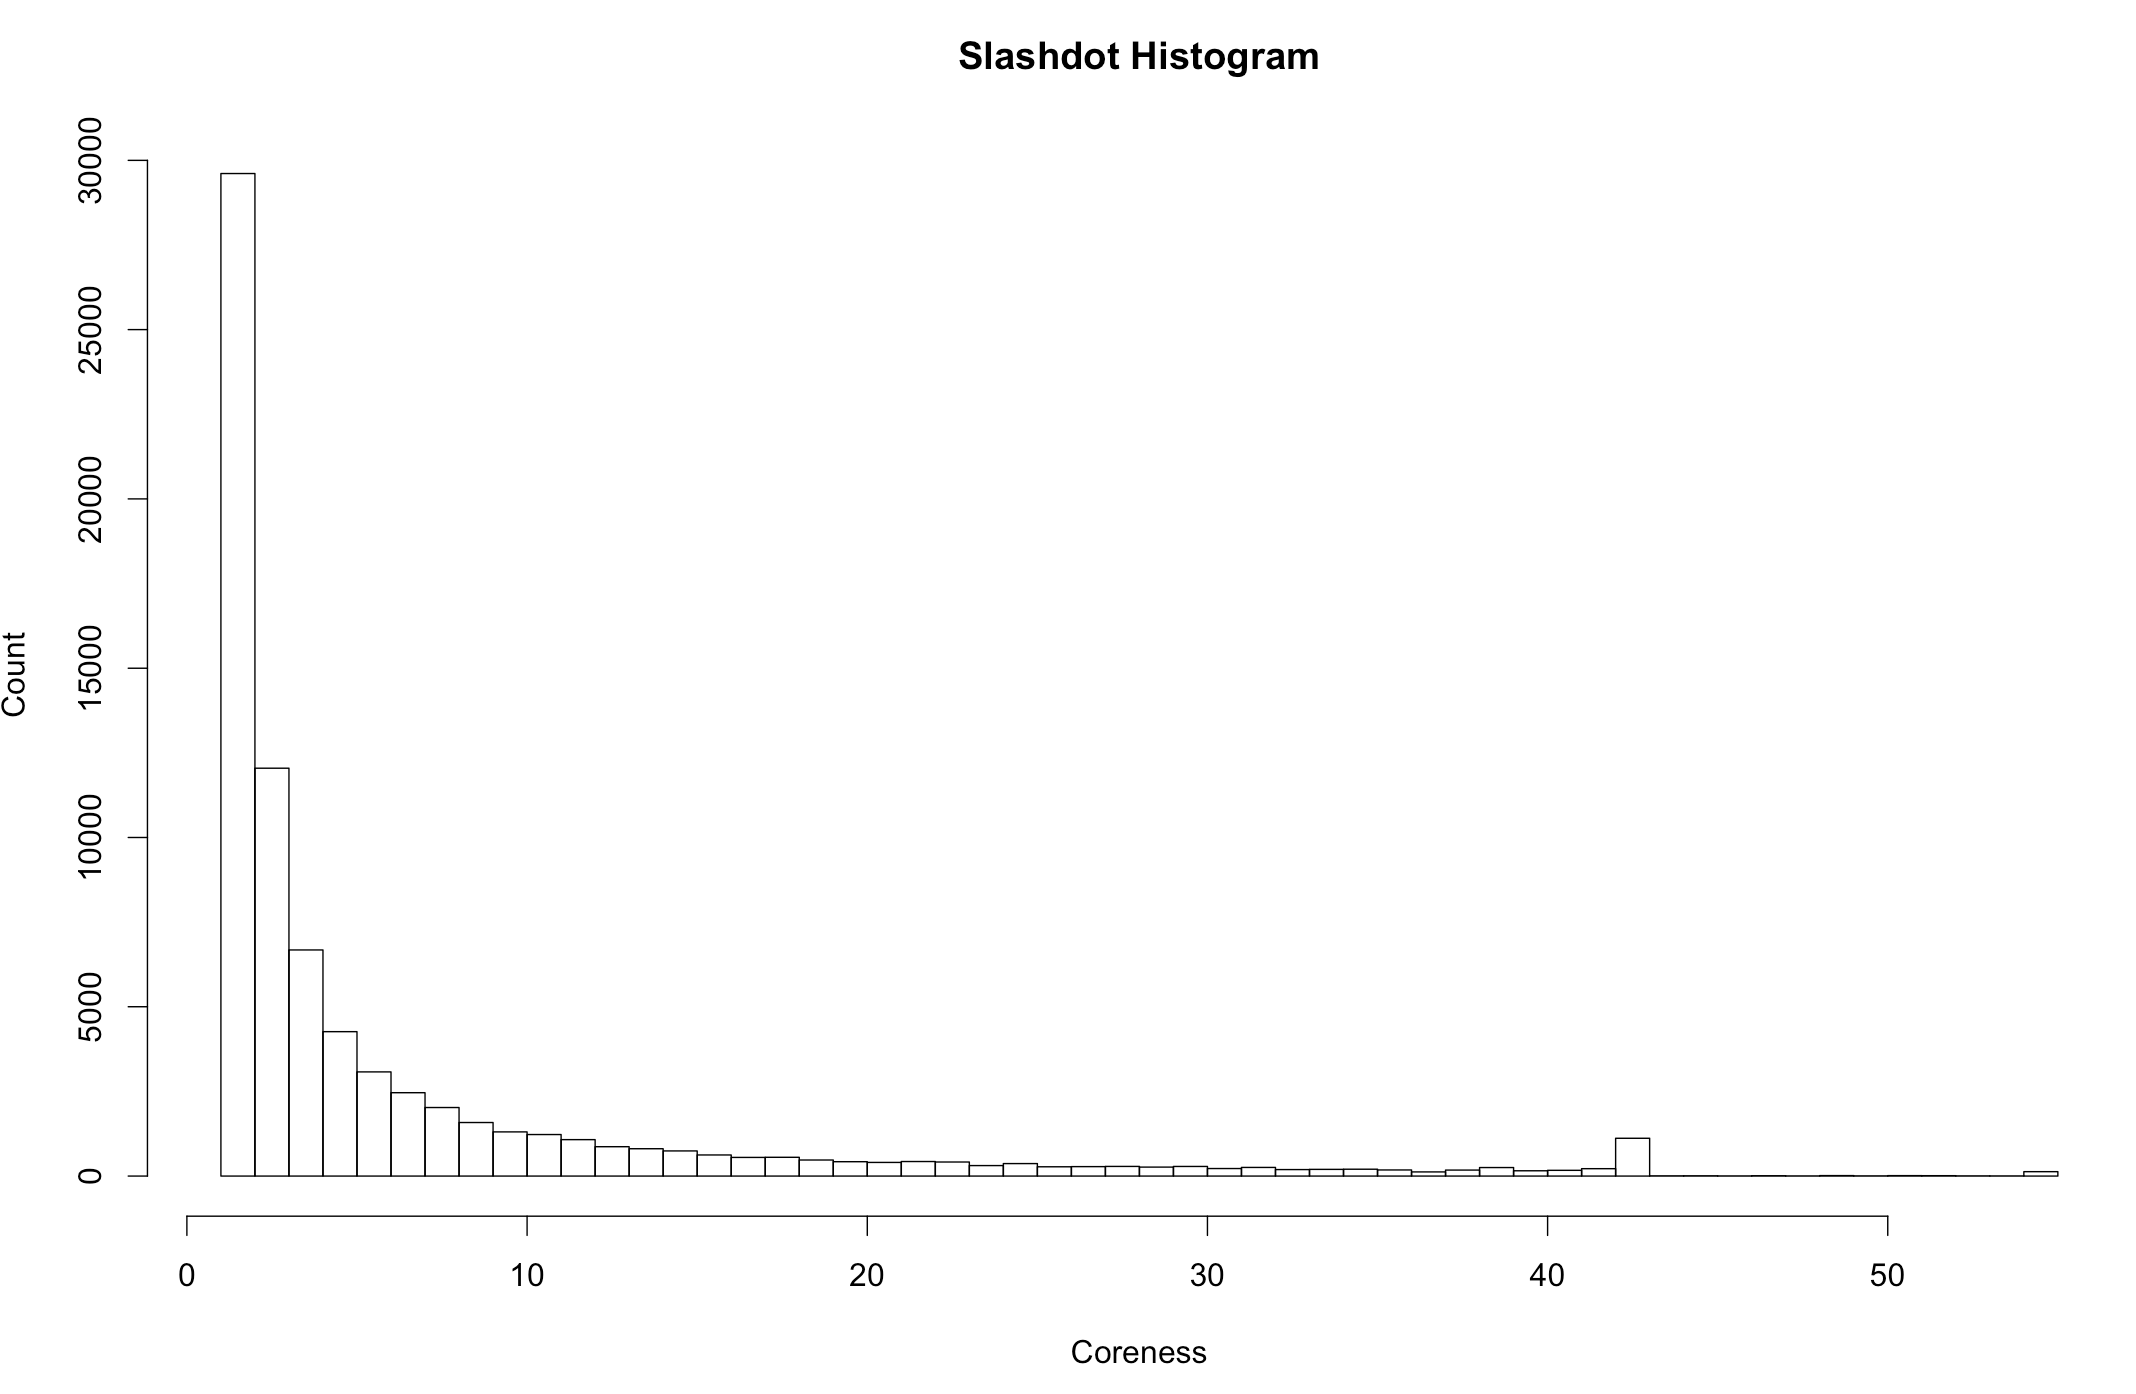
\includegraphics[width=\linewidth]{hist1}
  \caption{soc-Slashdot0811}
\endminipage\hfill
\minipage{0.48\textwidth}
  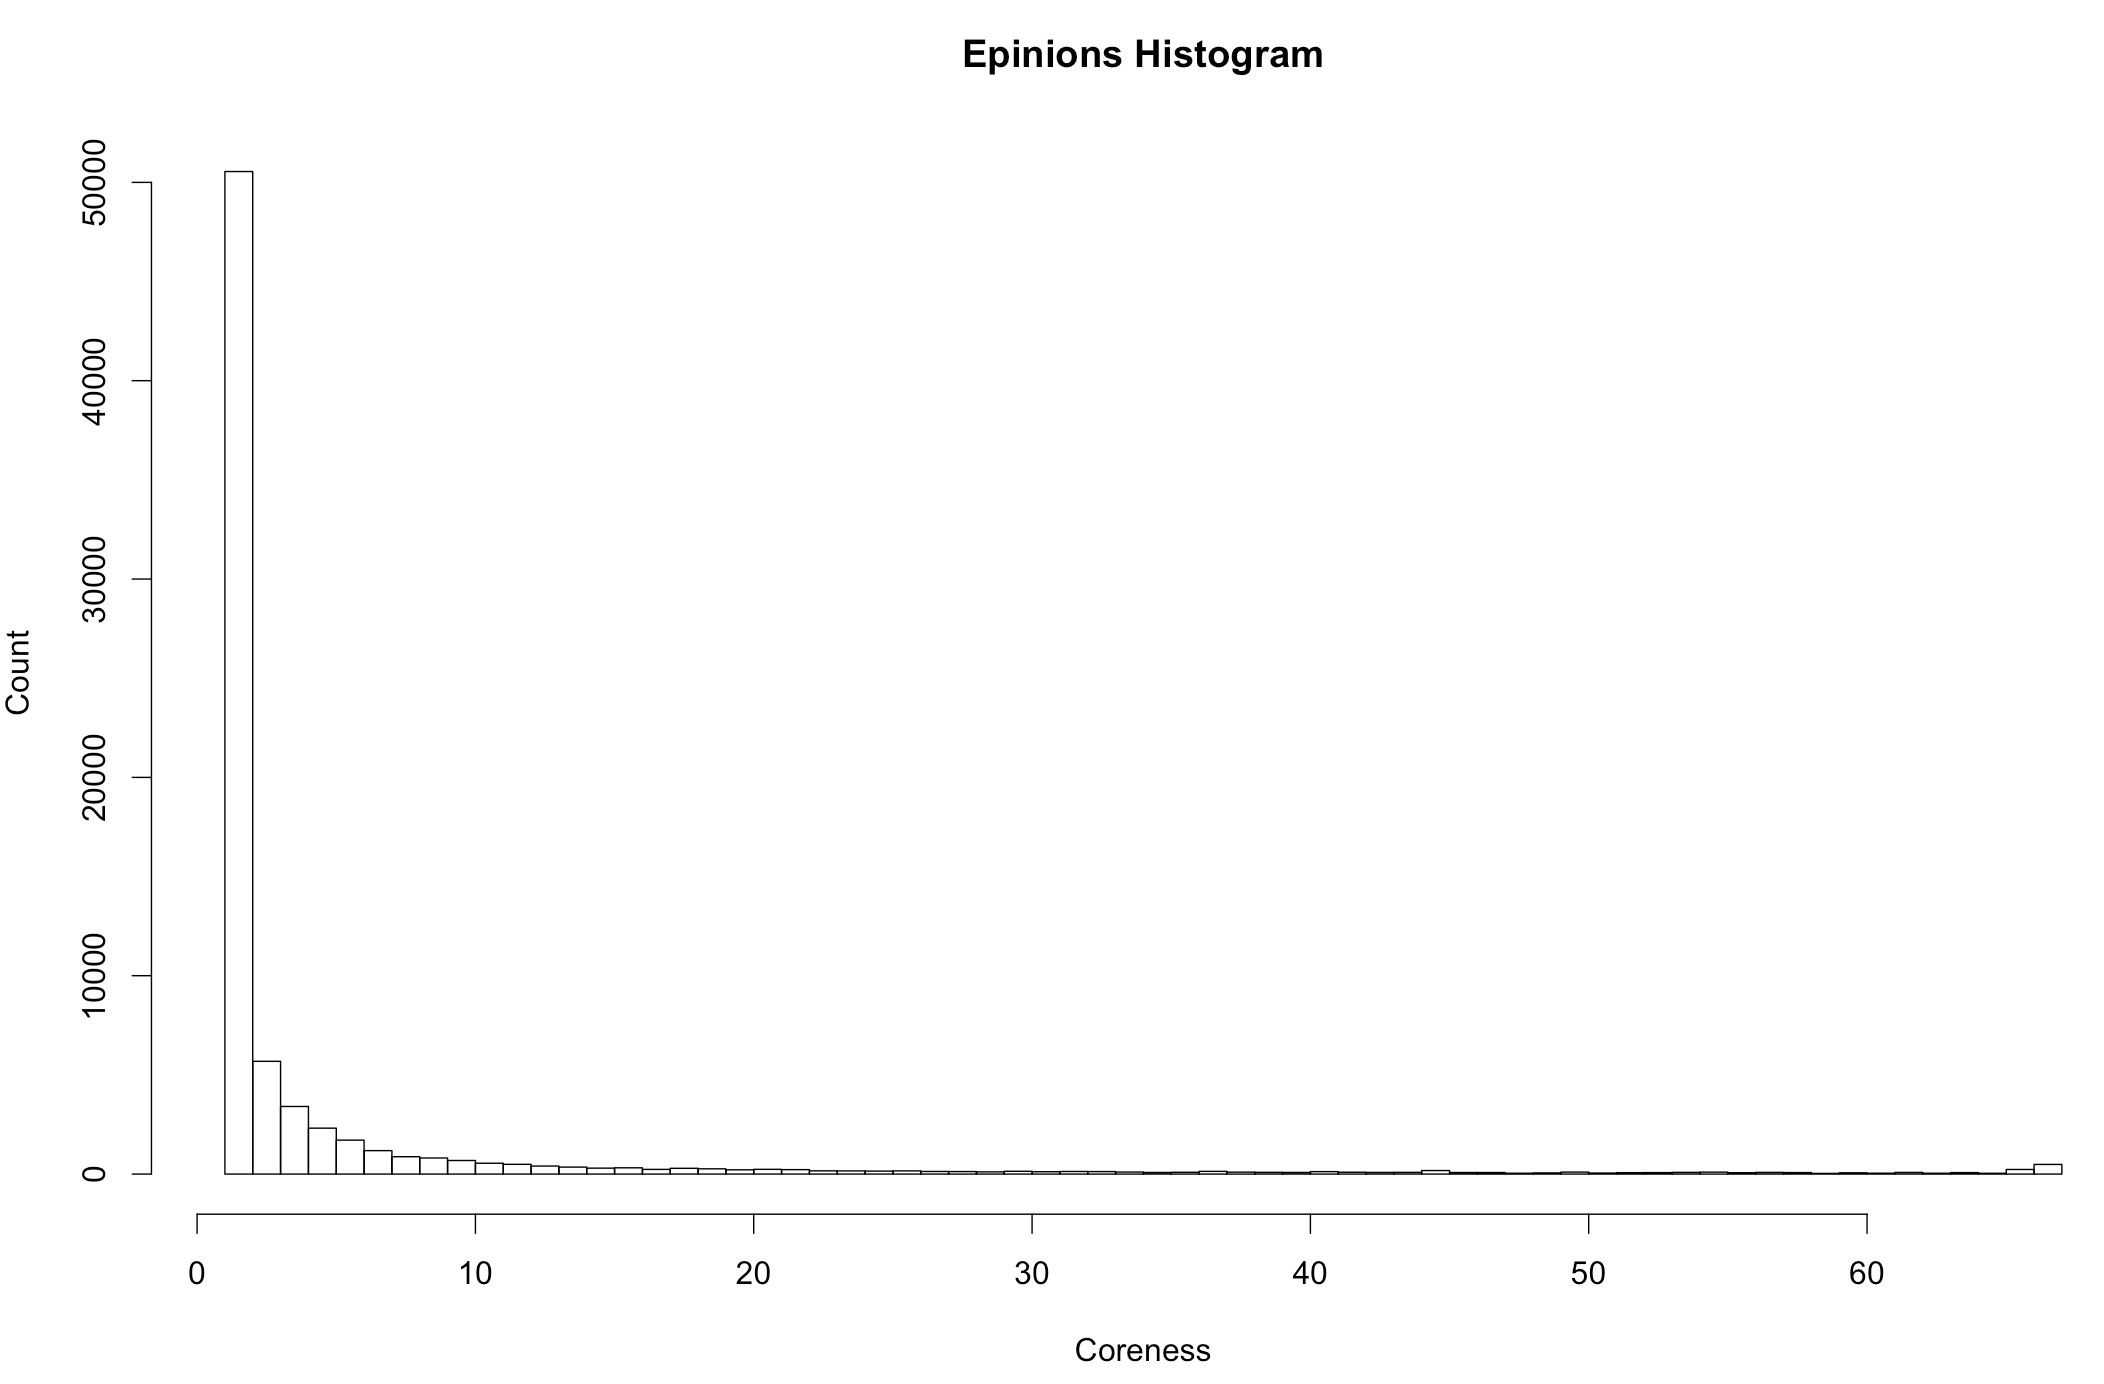
\includegraphics[width=\linewidth]{hist2}
  \caption{soc-Epinions1}
\endminipage
\end{figure}

\section{Phase2: Indexing}
    \label{sec:index}
    \subsection{Dataset}

We choose data from Stanford Large Network Dataset Collection, including social network, collaboration network and peer-to-peer network data.

\begin{table}[H]
	\begin{tabular}{| l | l | l | l | p{7cm} |}
	  \hline			
	  dataset & Type & Nodes & Edges & Description \\ \hline
	  ego-Facebook & Undirected & 4,039 & 88,234 & Social circles from Facebook (anonymized) \\ \hline
	  wiki-Vote & Directed & 7,115 & 103,689 & Wikipedia who-votes-on-whom networt \\ \hline
	  ca-GrQc & Undirected & 5,242 & 14,496 & Collaboration network of Arxiv General Relativity \\ \hline
	  ca-HepTh & Undirected & 9,877	& 25,998 & Collaboration network of Arxiv High Energy Physics Theory \\ \hline
	  p2p-Gnutella08 & Directed & 6,301 & 20,777 & Gnutella peer to peer network from August 8 2002 \\
	  \hline  
	\end{tabular}
\end{table}


\subsection{Performance}

In the following sections, we present the performance of different indexing methods \{non-clustering index on \texttt{source}, clustering index on \texttt{source}, composite index on \texttt{source} and \texttt{destination}\} $\times$ different node ordering methods \{random ordering, coreness ordering, pagerank ordering\}.

\subsubsection{Undirected Social Network: Facebook}

Facebook dataset has more edges and a long tail in degree distribution, hence it takes relatively longer run-time for our algorithms compared with other networks.

\begin{figure}[H]
\centering
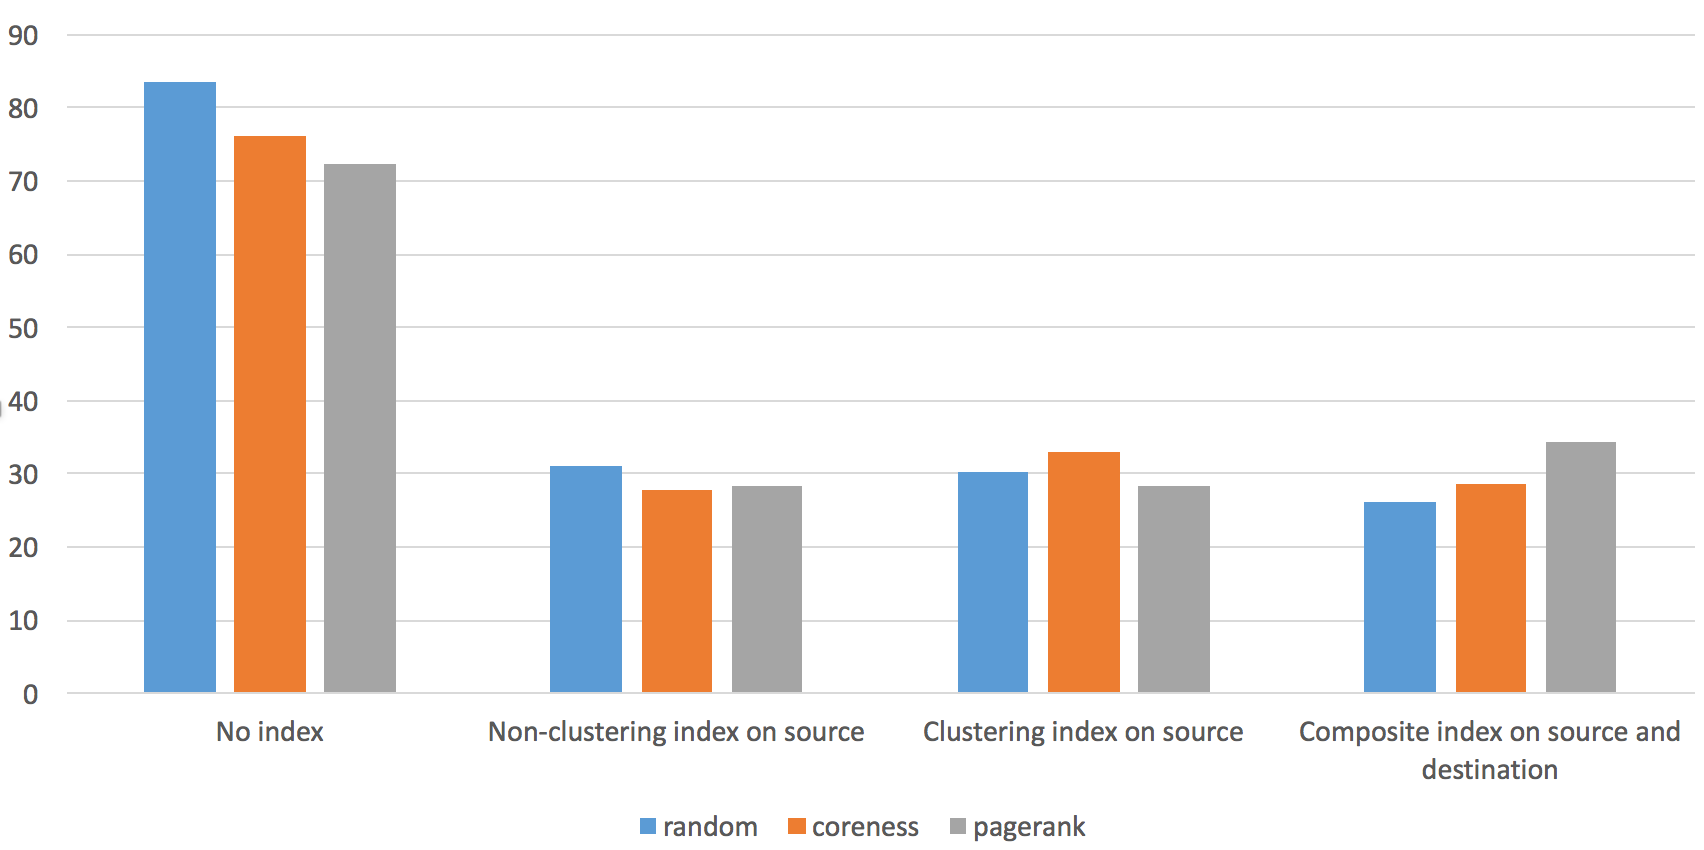
\includegraphics[width=0.8\linewidth]{fb}
\caption{Performance}
\end{figure}

\begin{figure}[H]
\centering
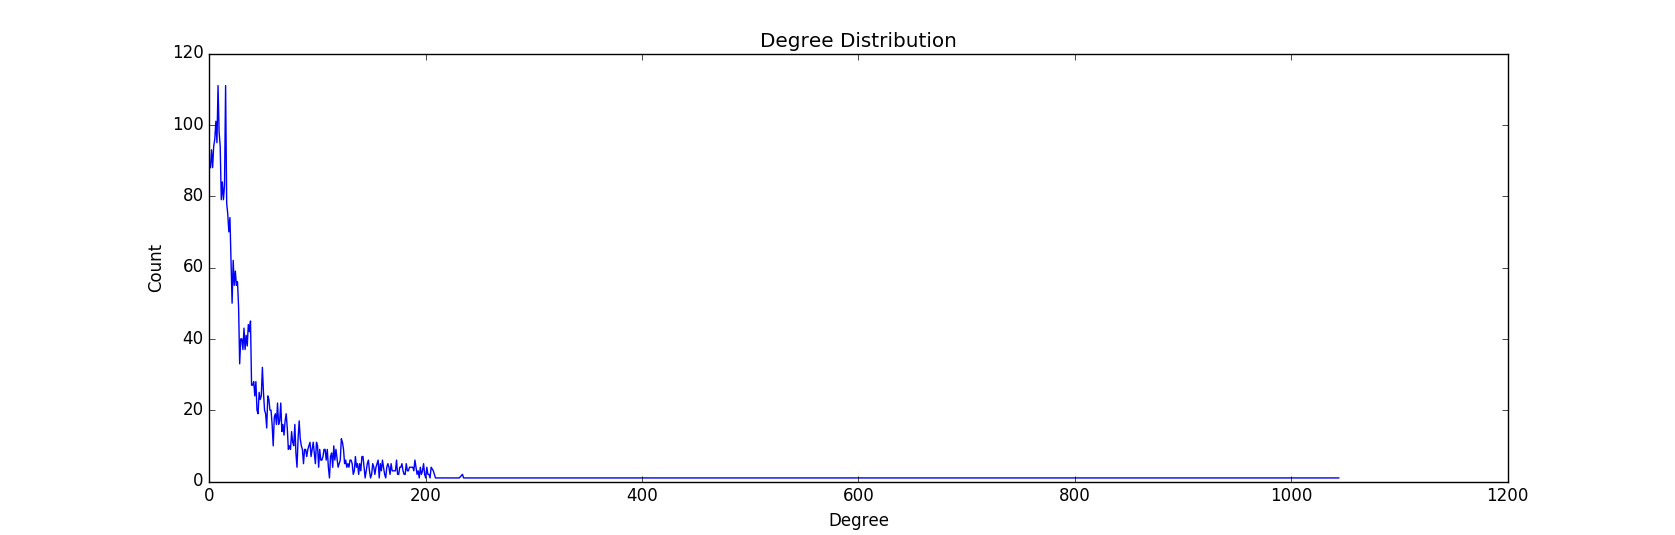
\includegraphics[width=1.0\linewidth]{fb_degree}
\caption{Degree Distribution}
\end{figure}

\begin{figure}[H]
\centering
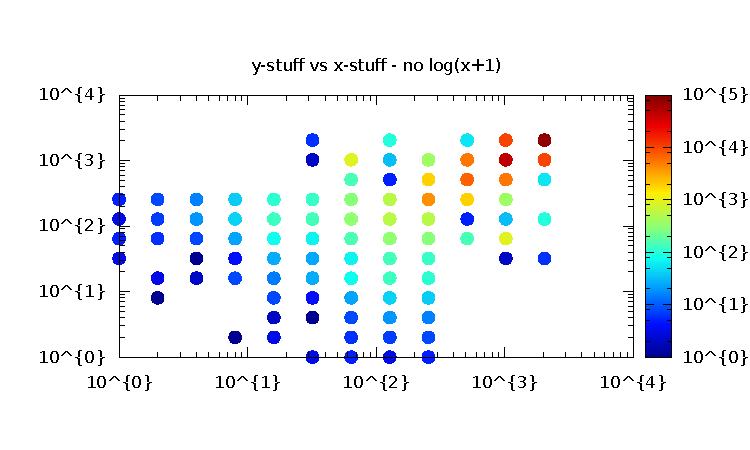
\includegraphics[width=0.8\linewidth]{core_scatter}
\caption{Scatter Plot}
\end{figure}

\subsubsection{Directed Social Network: Wiki Vote}

Wiki-Vote also belongs to social network dataset. From its degree distribution, we see it approximates power law and has relatively more edges. Majority of the nodes has small degrees while a few 'popular' has a degree over 1000. 

\begin{figure}[H]
\centering
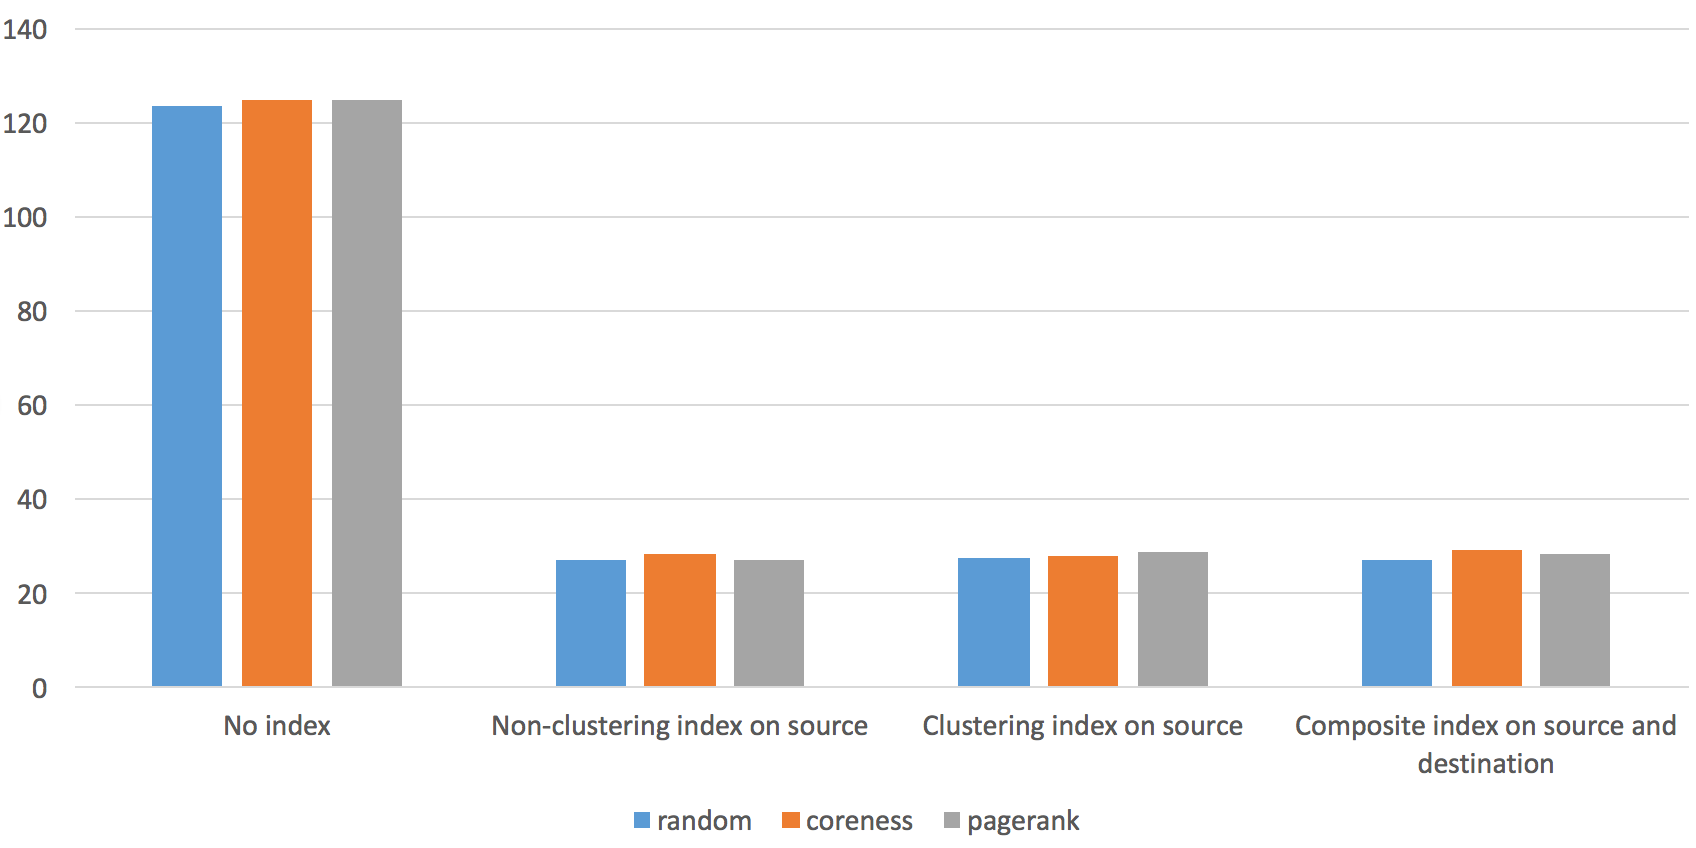
\includegraphics[width=0.8\linewidth]{wiki}
\caption{Performance}
\end{figure}

\begin{figure}[H]
\centering
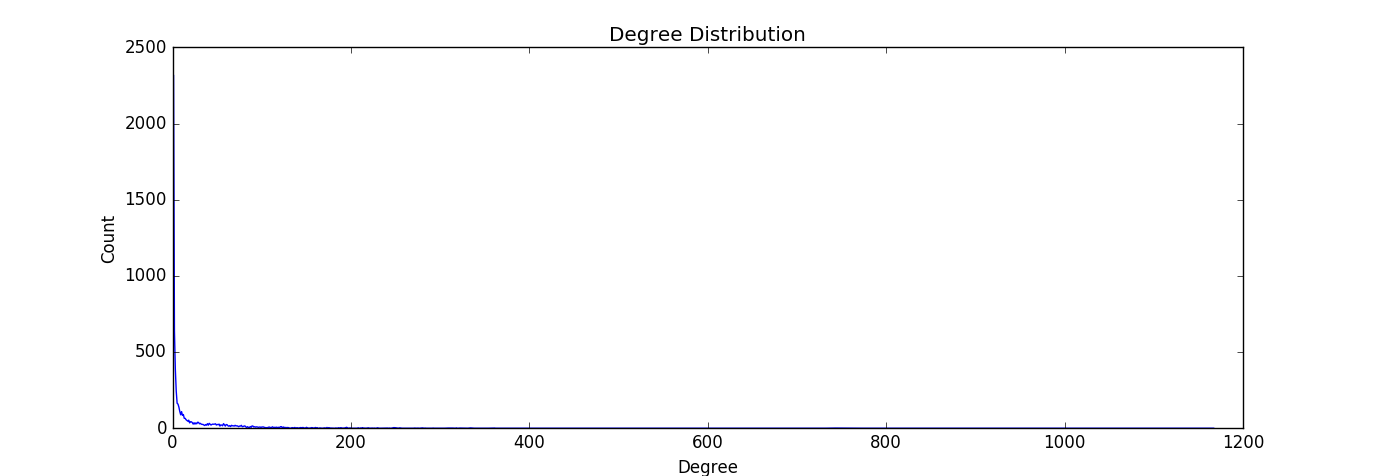
\includegraphics[width=1.0\linewidth]{wiki_degree}
\caption{Degree Distribution}
\end{figure}

\begin{figure}[H]
\centering
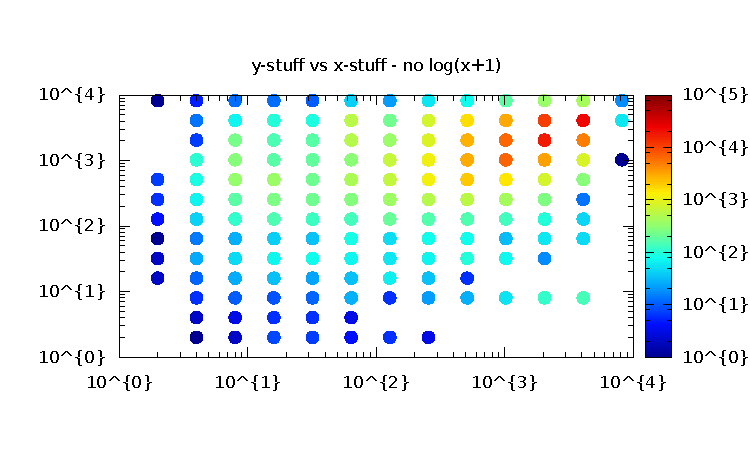
\includegraphics[width=0.8\linewidth]{wiki_scatter}
\caption{Scatter Plot}
\end{figure}

\subsubsection{Collaboration Network}
General Relativity and Quantum Cosmology collaboration network
\begin{figure}[H]
\centering
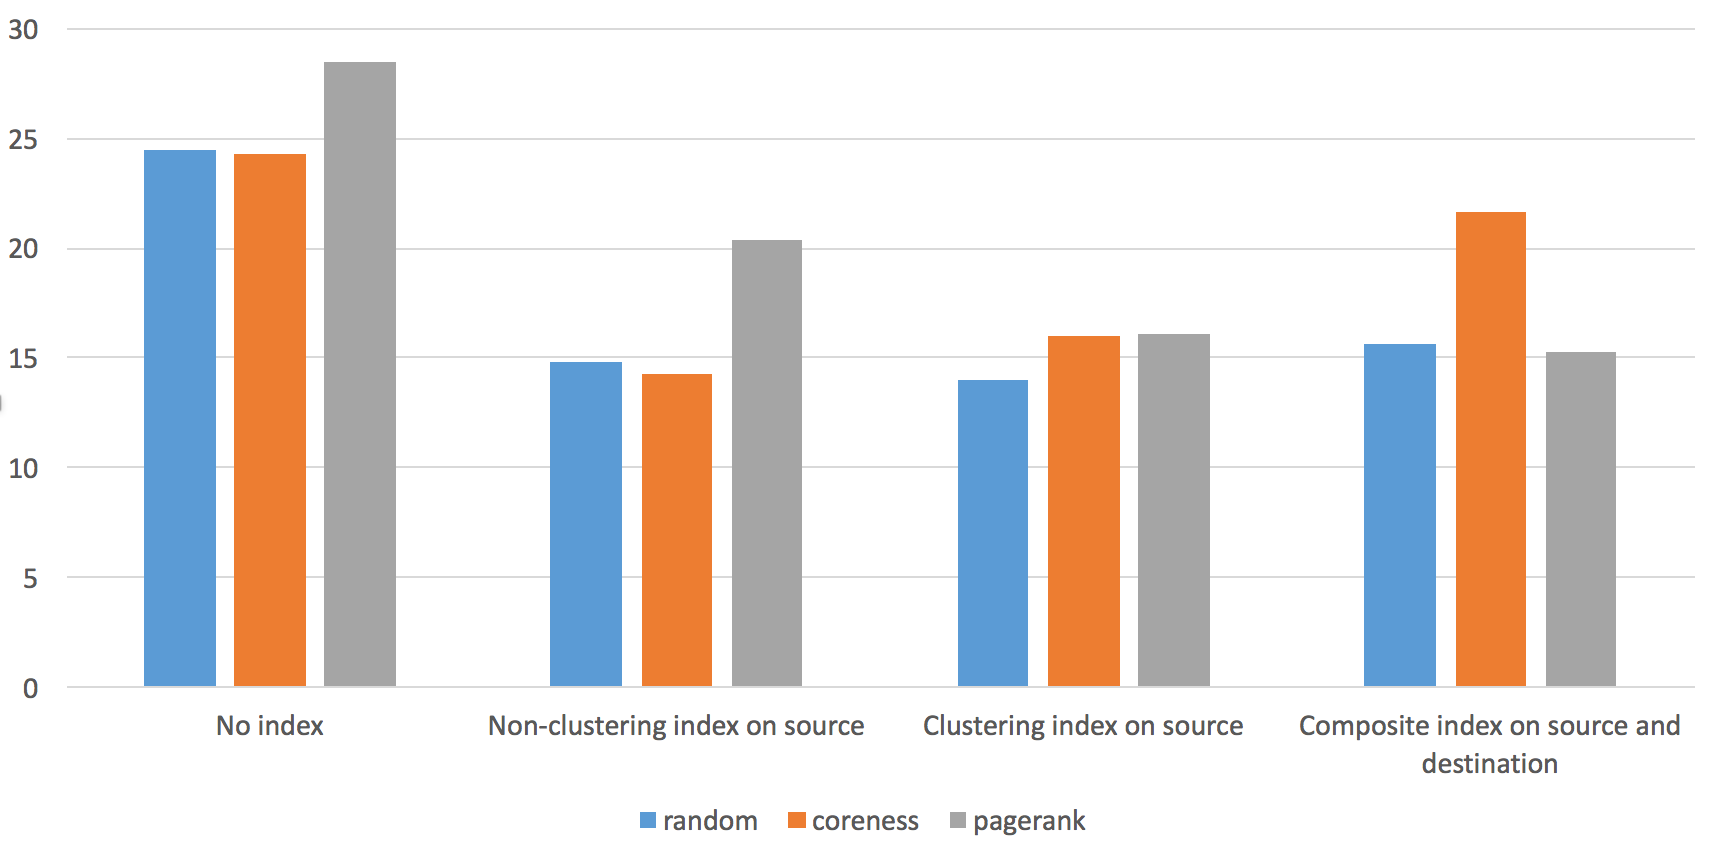
\includegraphics[width=0.8\linewidth]{co}
\caption{Performance}
\end{figure}
High Energy Physics - Theory collaboration network
\begin{figure}[H]
\centering
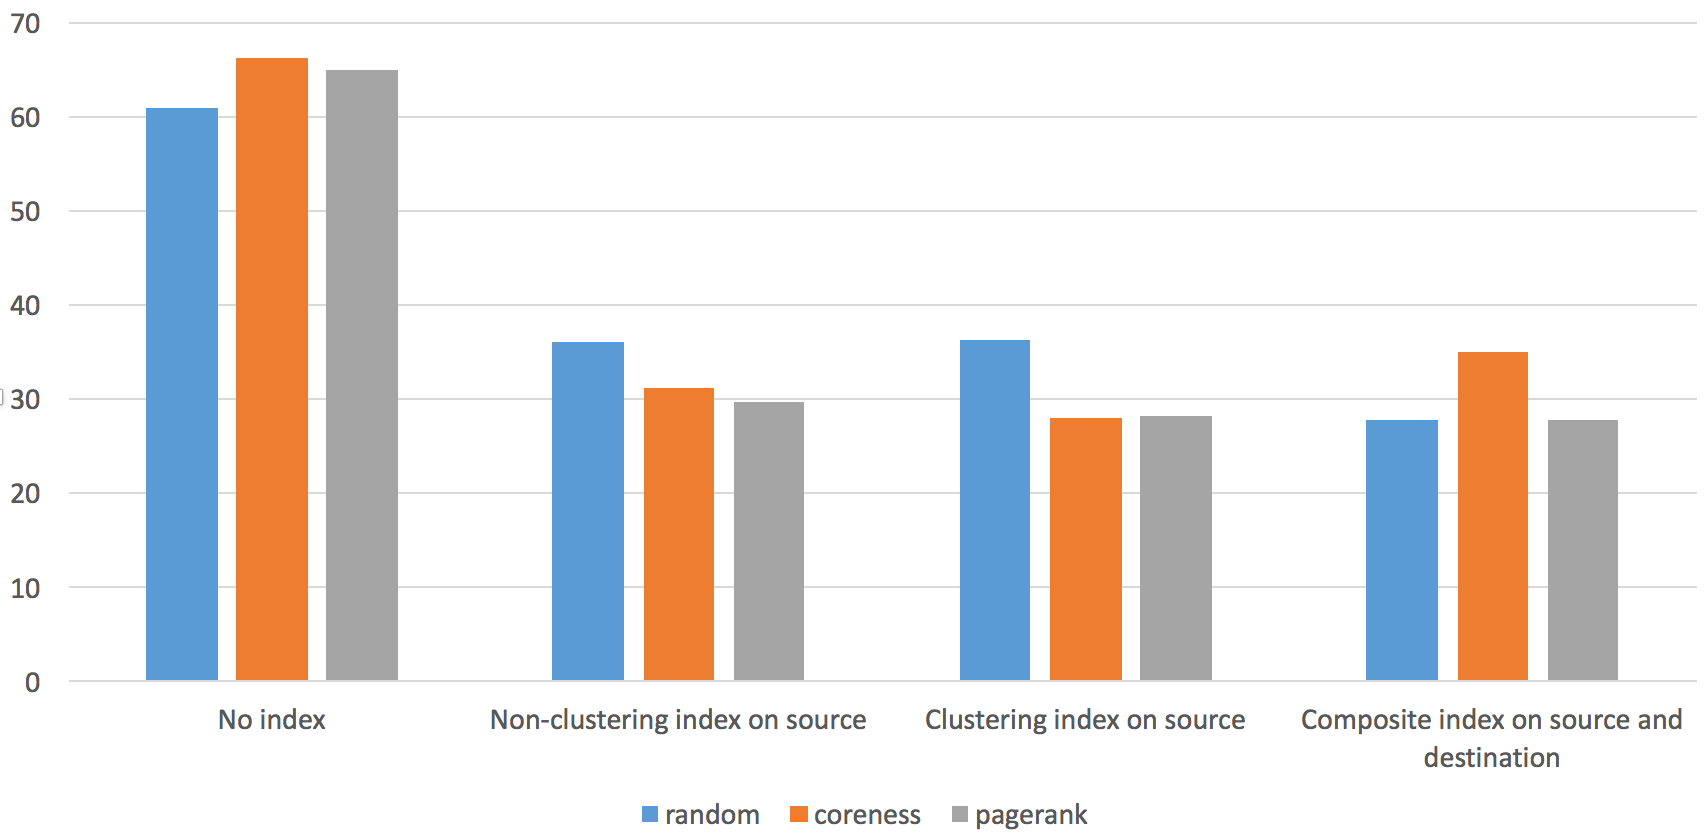
\includegraphics[width=0.8\linewidth]{ca}
\caption{Performance}
\end{figure}
Due to limited pages, we only list the degree distribution and scatter plot of General Relativity and Quantum Cosmology collaboration network as follows. They are quite similar.

\begin{figure}[H]
\centering
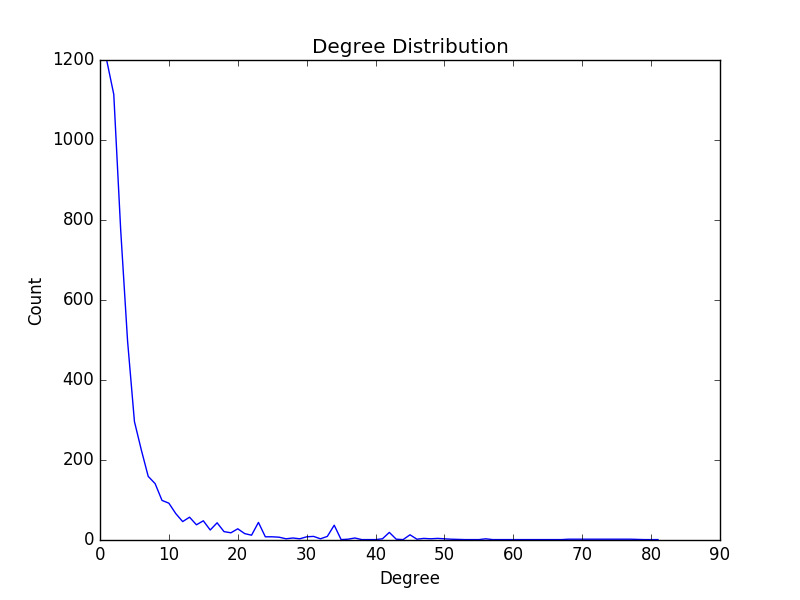
\includegraphics[width=0.6\linewidth]{ca_degree}
\caption{Degree Distribution}
\end{figure}

\begin{figure}[H]
\centering
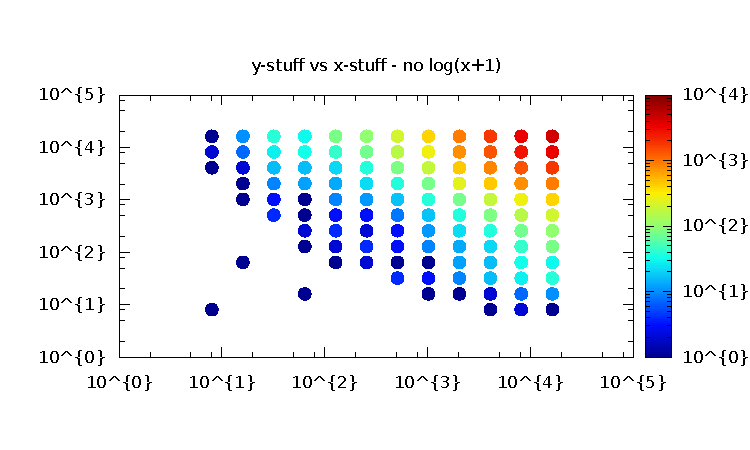
\includegraphics[width=0.8\linewidth]{ca_scatter}
\caption{Scatter Plot}
\end{figure}

\subsubsection{P2P Network}

\begin{figure}[H]
\centering
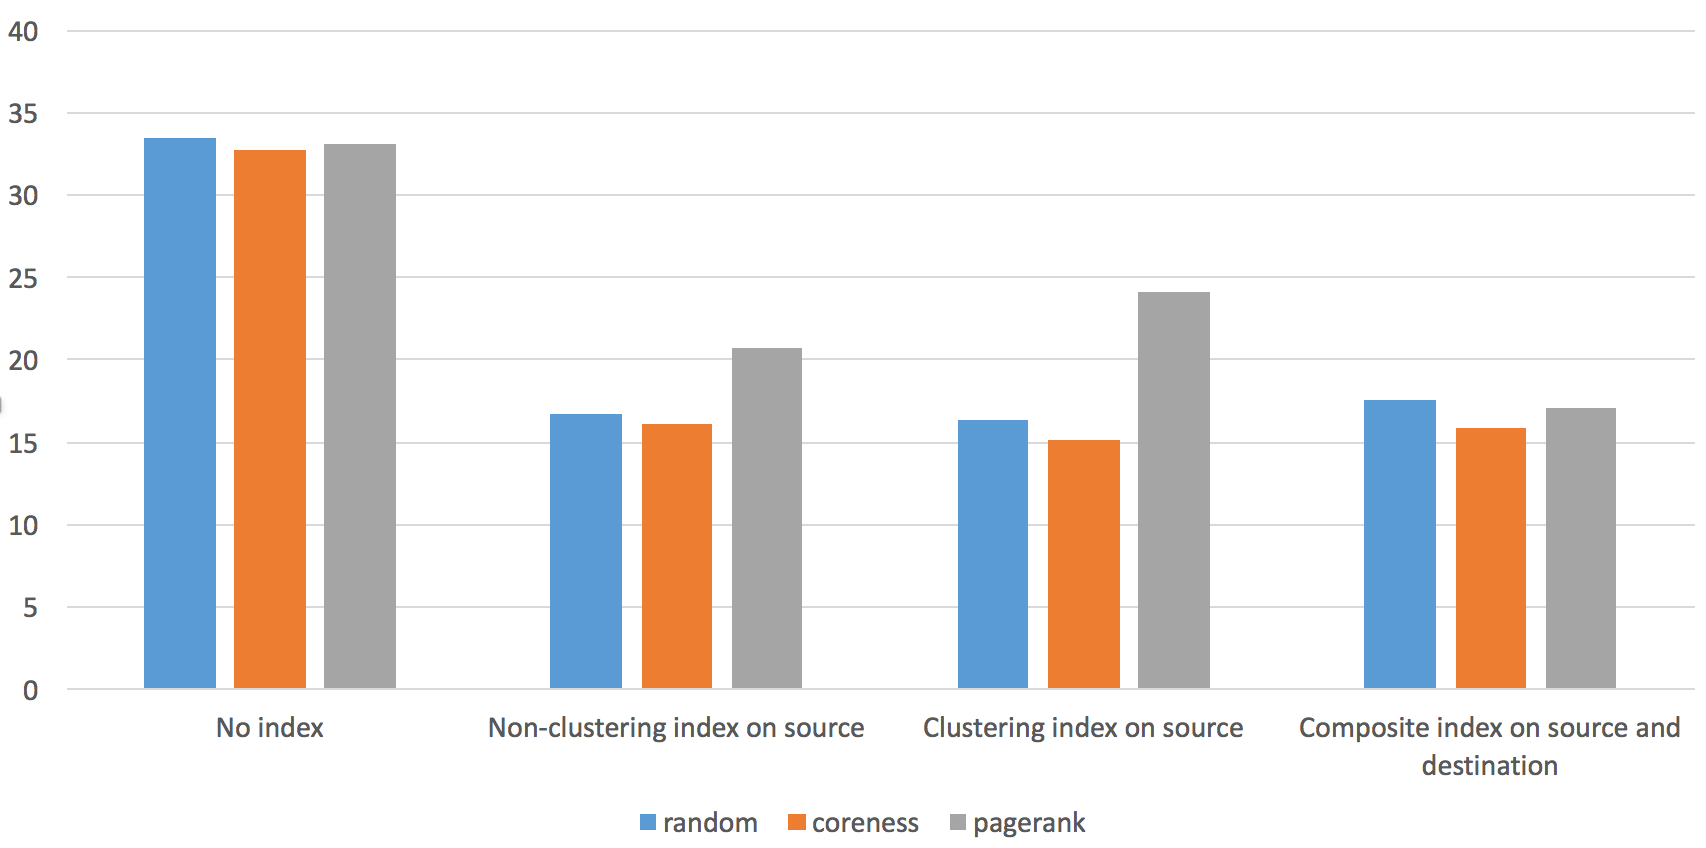
\includegraphics[width=0.8\linewidth]{p2p}
\caption{Performance}
\end{figure}

\begin{figure}[H]
\centering
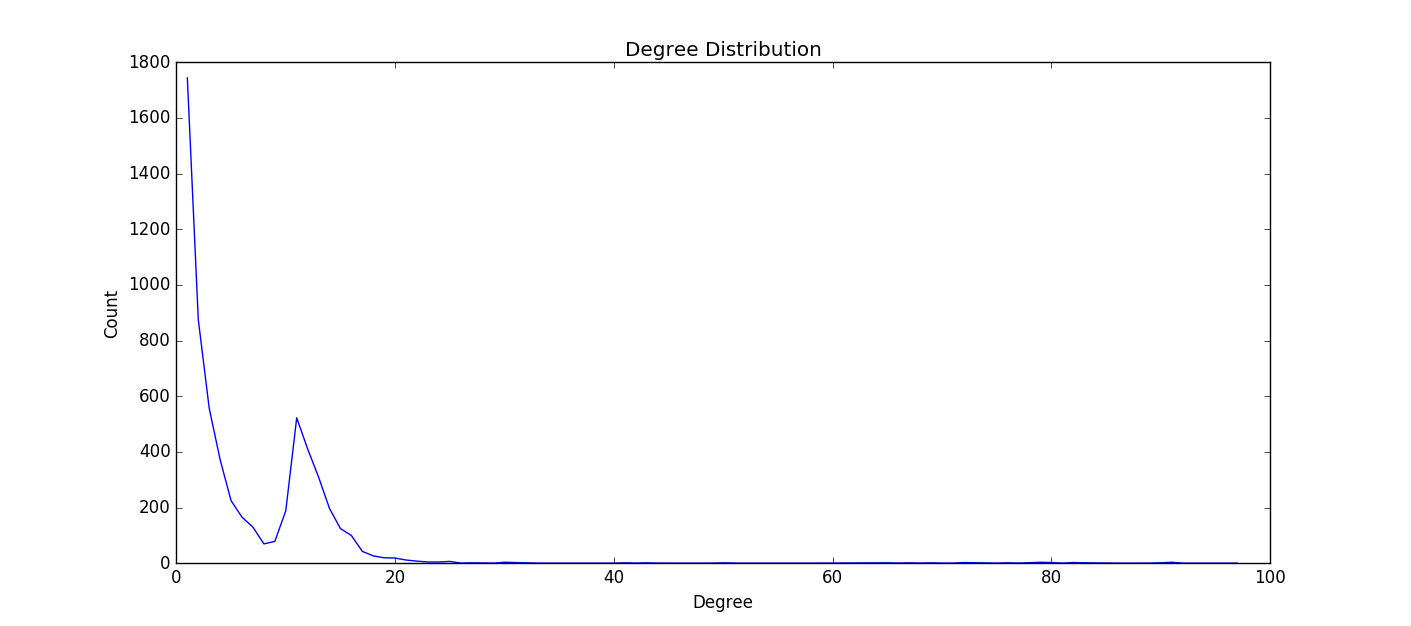
\includegraphics[width=0.8\linewidth]{p2p_degree}
\caption{Degree Distribution}
\end{figure}

\begin{figure}[H]
\centering
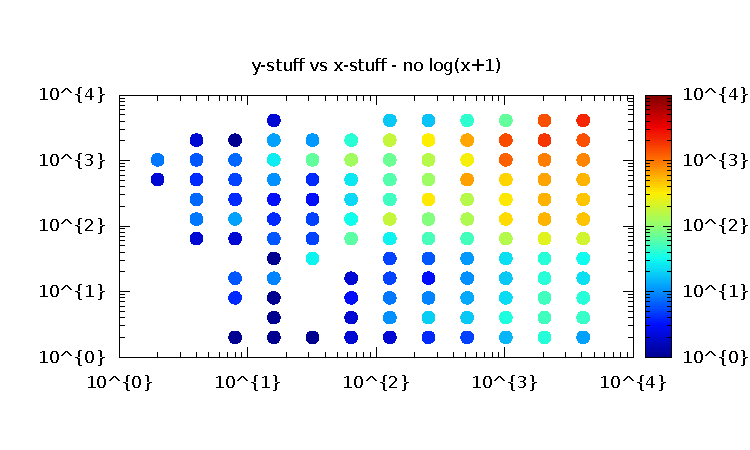
\includegraphics[width=0.8\linewidth]{p2p_scatter}
\caption{Scatter Plot}
\end{figure}

\subsection{Observation}

The most obvious result we can see from the experiment is that the running time get 2-4 times faster when using index. Degree of improvement depends on dataset types. \par

As for different types of index (clustering on source, non-clustering on source and composite index on source and destination), they all improve the running time and their impacts are similar. In some dataset e.g. Facebook, data with composite indexes run slightly faster. In other dataset like wiki-Vote ranked by coreness, clustering index gives a slightly better performance. So the performance of different indexes is dependent on dataset. \par

Clustering index stores actual rows on the disc and search for actual rows while non-clustered index store pointers and pointers point to where actual rows are stored. Generally clustering index would provide a faster way of searching, but in our experiment, we not only have searching, but also a huge amount of work of deleting, which may slow down using clustering index. \cite{MSR} \par

We also experiment on preprocessing the data, ranking the source node id in the initial dataset by coreness and page rank. And we find out there is not much difference in running time when we reorder the dataset first. Adding indexes to the reordered dataset also show similar trend as the original random data. \par

Another interesting finding is that the five datasets we use have different number of nodes and edges, but the running time of the algorithm is not proportional to the number of nodes. For example, ca-HepTh dataset has 9877 nodes while Facebook has 4024 nodes; however, the raw running time of Facebook is 83s while ca-HepTh is 61s. But when we look at their edges, we find that the edges in Facebook is 88234, almost 4 times the edges in ca-HepTh. So we may say that the number of edges determines the running time. In addition, as we look at dataset wiki-Vote, it has the largest number of edges: 103,689, and we see the raw running time is longer than the other datasets. Surprisingly, after adding index to it, the running time decreases dramatically from 123s to 27s, even shorter than the other datasets. \par


\section{Phase3: Discovery}
    \label{sec:final}
    \subsection{User-manual documentation on k-degeneracy}
This section describes the idea of k-core and the implementation of analyzing the degeneracy of of a graph using SQL.\par

First, we look at the definition of coreness: (definitions come from project writeup) A node in an undirected graph has coreness k, if it has k or more neighbors that have coreness k or higher, and k is the maximum such integer for node n. After we know the coreness of each node in the graph, we can get the degeneracy of a graph. The formal definition is: Degeneracy D of a graph is the highest coreness among the nodes of thegraph.\par

Now we have seen the definition of degeneracy, so the general idea of finding the coreness of each node is described below: iterate from k = 1, and we want to find nodes whose coreness = k; for each k, find those nodes who has neighbors less than or equal to k, so those numbers are of coreness k; delete those nodes from the graph; repeat until we can not find any of the node who has neighbors $\le$ k, all the nodes left must have coreness greater than k, so we increase k by 1; terminate when there is no node in the graph.\par

Part of the SQL code are provided below:\par
\begin{lstlisting}
-- 1. start from k = 1, loop when we can still find nodes with neighbors <= k
--     create a temp table to store all nodes that we find with neighbors <= k
INSERT INTO TMP_TABLE
SELECT src_id, COUNT(*) AS neighbor FROM GM_TABLE
GROUP BY src_id HAVING count(*) <= k;
                 
-- 2. check if there is no nodes satisfying the conditions, increase k by 1 and continue from the start of the loop
SELECT COUNT(*) FROM TMP_TABLE;
-- if count is 0, k += 1 and continue

-- 3. save those nodes to a permanent table with their coreness
INSERT INTO GM_KCORE
SELECT src_id, k AS coreness FROM TMP_TABLE;

-- 4. delete those nodes from the original table
DELETE FROM GM_TABLE
WHERE src_id IN (SELECT src_id FROM TMP_TABLE);
DELETE FROM GM_TABLE
WHERE dst_id IN (SELECT src_id FROM TMP_TABLE);
	
-- 5. terminate if there is no node in the original table
SELECT COUNT(*) FROM GM_TABLE;
-- if count is 0, break the loop
		
-- 6. calculate the degeneracy of the graph, which is the largest coreness among all nodes
SELECT MAX(coreness) FROM GM_KCORE;
\end{lstlisting}

\subsection{Dataset}

Our datasets are adopted from SNAP (Stanford Large Network Dataset Collection) \\
\url{http://snap.stanford.edu/data/index.html}.

\begin{table}[H]
	\begin{tabular}{| l | l | l | l | p{8cm} |}
	  \hline			
	  dataset & Type & Nodes & Edges & Description \\ \hline

	  Facebook & Undirected & 4,039 & 88,234 & \textbf{Social network} Social circles from Facebook (anonymized) \\ \hline

	  soc-Slashdot0811 & Directed & 77,360 & 905,468 & \textbf{Social network} Slashdot social network from November 2008 \\ \hline

	  soc-Slashdot0922 & Directed & 82,168 & 948,464 & \textbf{Social network} Slashdot social network from February 2009 \\ \hline

	  soc-Epinions1 & Directed & 75,879	& 508,837 & \textbf{Social network} Who-trusts-whom network of Epinions.com \\ \hline

	  wiki-Vote	& Directed & 7,115 & 103,689 & \textbf{Wikipedia social network} Wikipedia who-votes-on-whom network \\ \hline

	  email-Enron & Undirected & 36,692 & 183,831 & \textbf{Communication network} Email communication network from Enron \\ \hline
	  
	  ca-HepTh & Undirected & 9,877	& 25,998 & \textbf{Collaboration network} of Arxiv High Energy Physics Theory \\ \hline

	  ca-GrQc & Undirected & 5,242 & 14,496 & \textbf{Collaboration network} of Arxiv General Relativity \\ \hline

	  ca-AstroPh & Undirected & 18,772 & 198,110 & \textbf{Collaboration network} of Arxiv Astro Physics \\ \hline

	  p2p-Gnutella24 & Directed & 26,518 & 65,369 & \textbf{P2P Network} Gnutella peer to peer network from August 24 2002 \\ \hline

	  p2p-Gnutella25 & Directed & 22,687 & 54,705 & \textbf{P2P Network} Gnutella peer to peer network from August 25 2002 \\ \hline

	  oregon1-010331 & Undirected & 10,670 & 22,002 & \textbf{Autonomous system} peering information inferred from Oregon route-views from March 31 \\ \hline

	  oregon1-010519 & Undirected & 11,051 & 22,724 & \textbf{Autonomous system} peering information inferred from Oregon route-views from May 19 \\ \hline

	  cit-HepPh & Directed & 34,546 & 421,578 & \textbf{Citation network} Arxiv High Energy Physics paper citation network \\ \hline

	  cit-HepTh & Directed & 27,770 & 352,807 & \textbf{Citation network} Arxiv High Energy Physics paper citation network \\
	  
	  \hline  
	\end{tabular}
\end{table}

\subsection{Results}

All the graphs shown below are in log-log scale.

\subsubsection{Degree Distribution}

Scatter plot \quad x-axis: degree \quad y-axis: count

\begin{figure}[H]
\minipage{0.33\textwidth}
  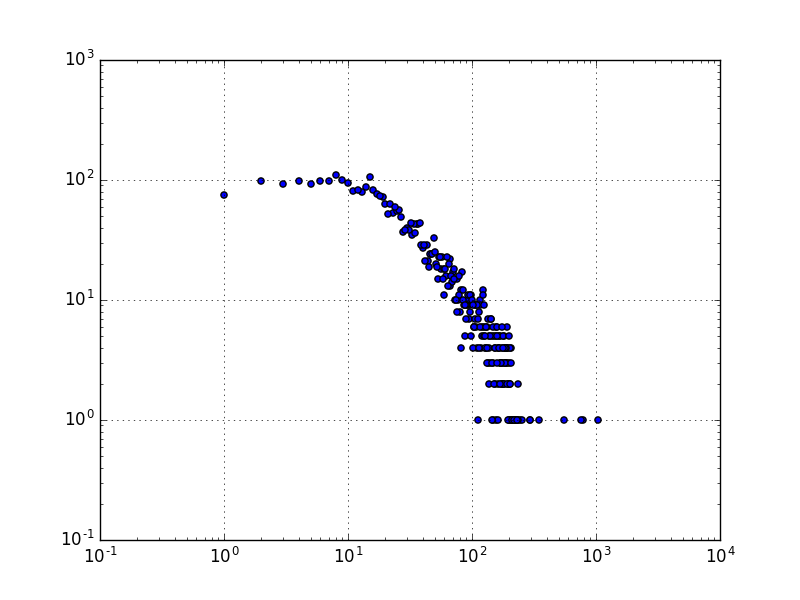
\includegraphics[width=\linewidth]{img/facebook/degree_dist.png}
  \caption*{Facebook}
\endminipage\hfill
\minipage{0.33\textwidth}
  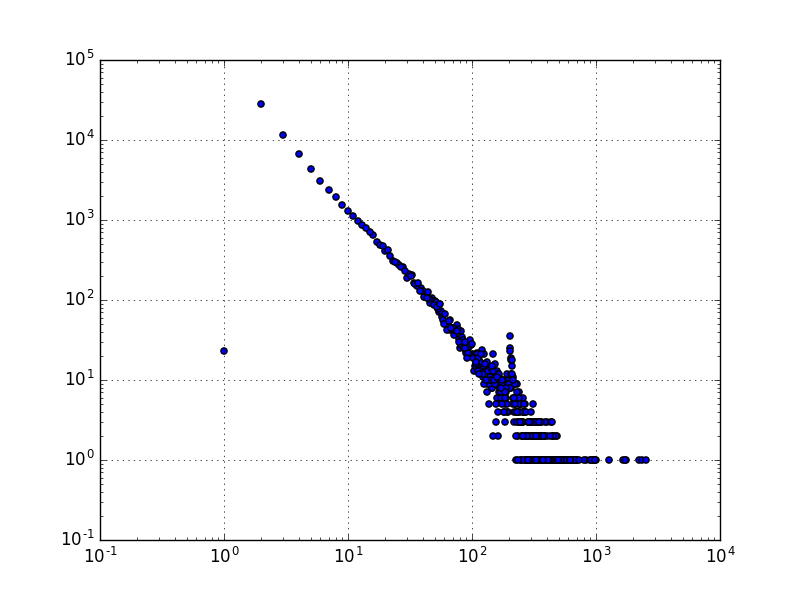
\includegraphics[width=\linewidth]{img/slashDot/degree_dist.png}
  \caption*{soc-Slashdot0811}
\endminipage\hfill
\minipage{0.33\textwidth}
  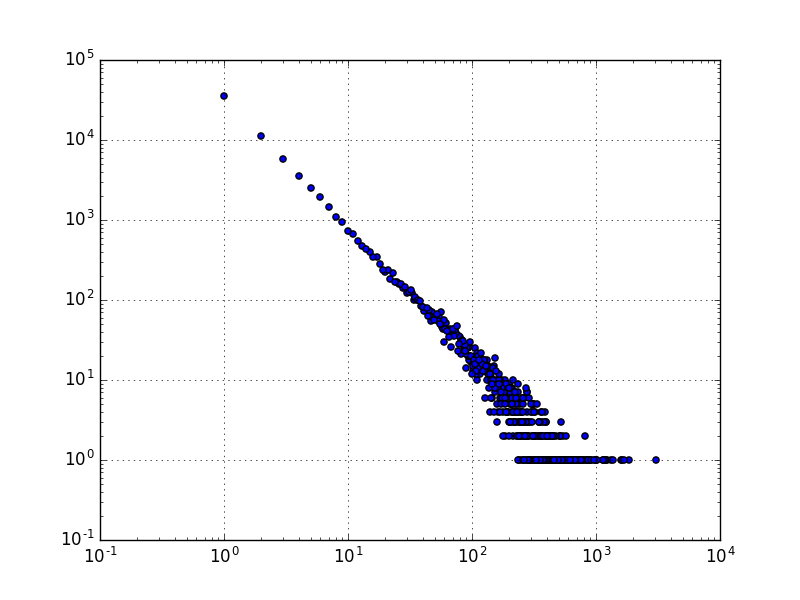
\includegraphics[width=\linewidth]{img/soc-E/degree_dist.png}
  \caption*{soc-Epinions1}
\endminipage
\end{figure}

\begin{figure}[H]
\minipage{0.33\textwidth}
  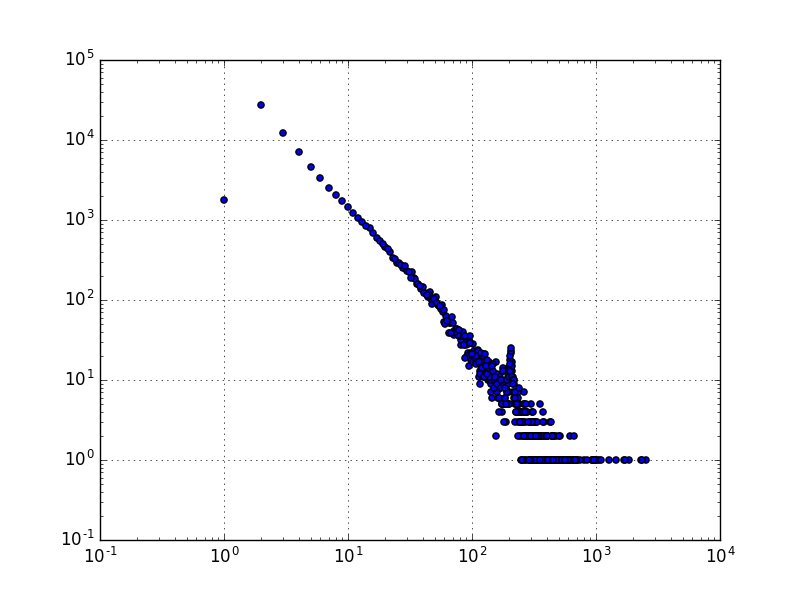
\includegraphics[width=\linewidth]{img/slashDot09/degree_dist.png}
  \caption*{soc-Slashdot0922}
\endminipage\hfill
\minipage{0.33\textwidth}
  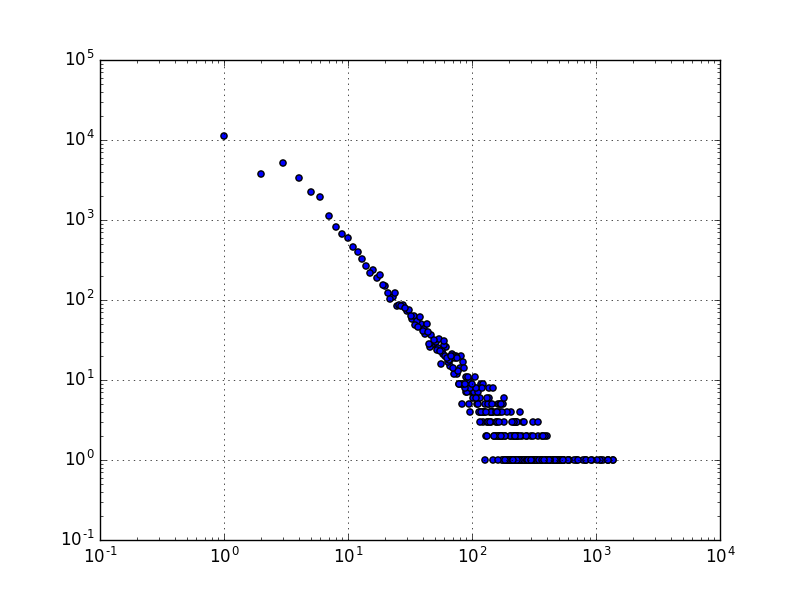
\includegraphics[width=\linewidth]{img/email/degree_dist.png}
  \caption*{email-Enron}
\endminipage\hfill
\minipage{0.33\textwidth}
  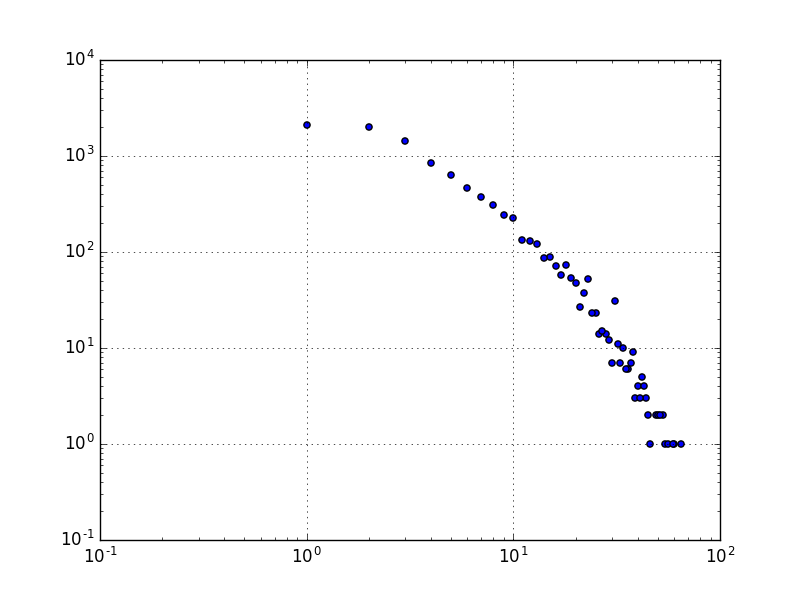
\includegraphics[width=\linewidth]{img/ca-HepTh/degree_dist.png}
  \caption*{ca-HepTh}
\endminipage
\end{figure}

\begin{figure}[H]
\minipage{0.33\textwidth}
  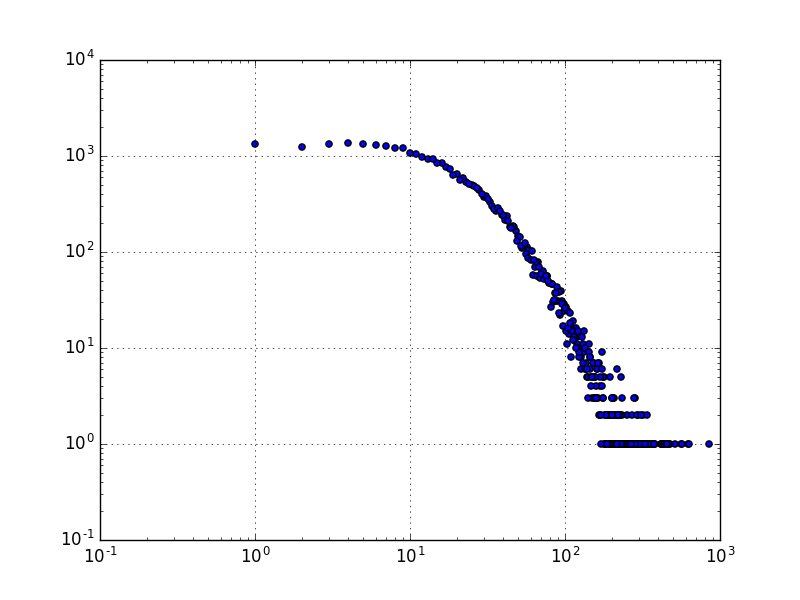
\includegraphics[width=\linewidth]{img/cit-HepPh/degree_dist.png}
  \caption*{cit-HepPh}
\endminipage\hfill
\minipage{0.33\textwidth}
  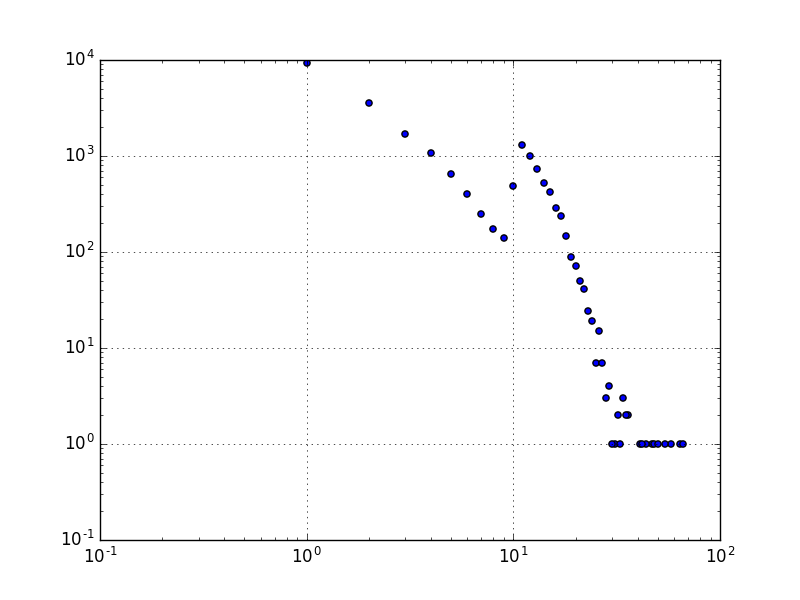
\includegraphics[width=\linewidth]{img/p2p-Gnutella25/degree_dist.png}
  \caption*{p2p-Gnutella25}
\endminipage\hfill
\minipage{0.33\textwidth}
  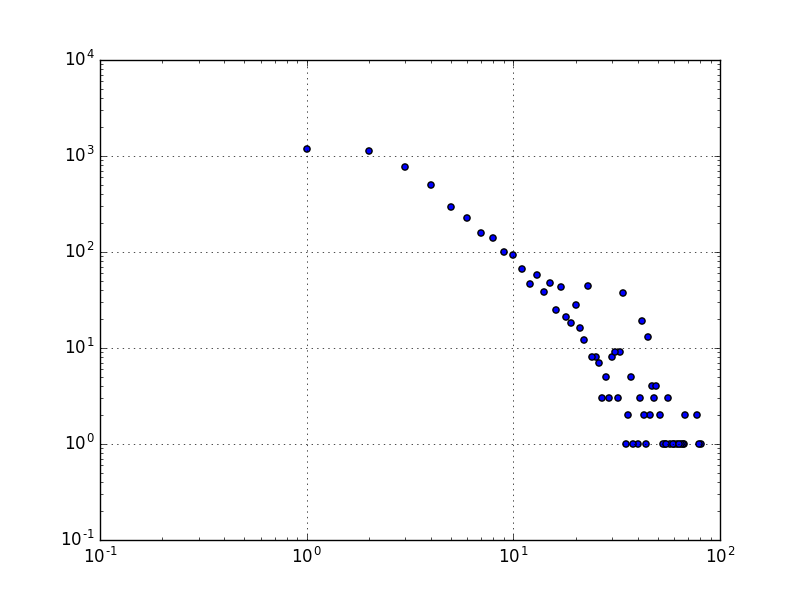
\includegraphics[width=\linewidth]{img/ca-GrQc/degree_dist.png}
  \caption*{ca-GrQc}
\endminipage
\end{figure}

\begin{figure}[H]
\minipage{0.33\textwidth}
  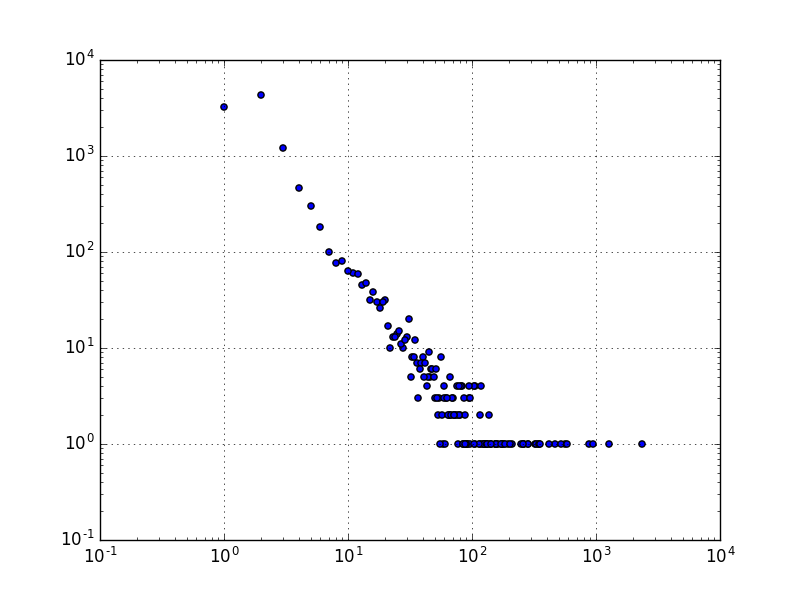
\includegraphics[width=\linewidth]{img/oregon-010331/degree_dist.png}
  \caption*{Oregon1-010331}
\endminipage\hfill
\minipage{0.33\textwidth}
  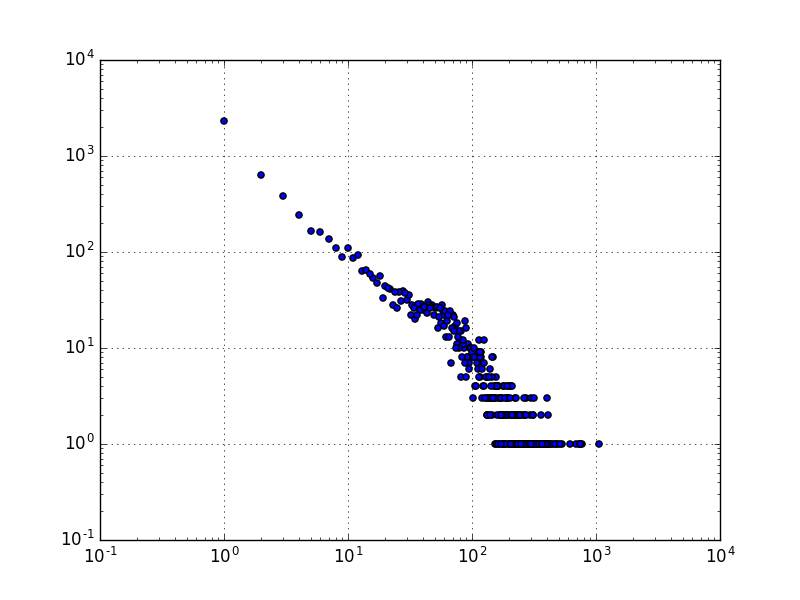
\includegraphics[width=\linewidth]{img/wiki-Vote/degree_dist.png}
  \caption*{wiki-Vote}
\endminipage\hfill
\minipage{0.33\textwidth}
  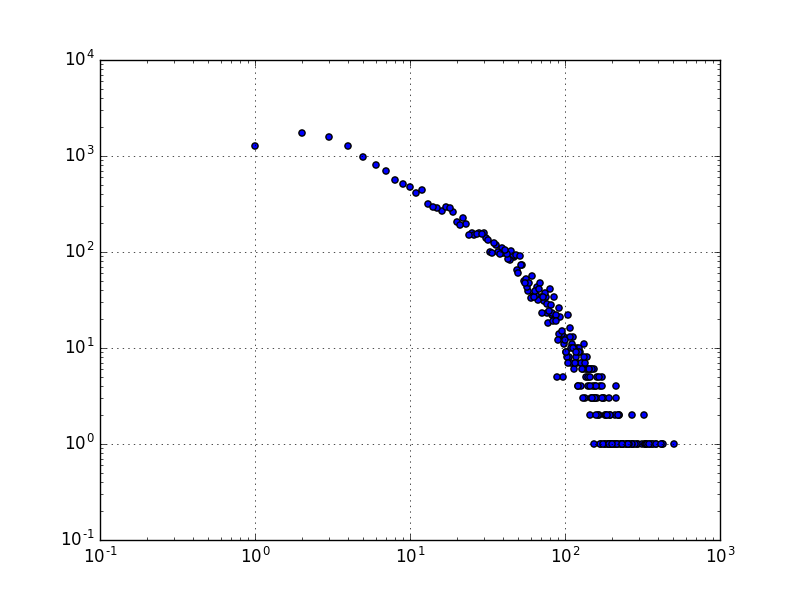
\includegraphics[width=\linewidth]{img/ca-Astro/degree_dist.png}
  \caption*{ca-Astro}
\endminipage
\end{figure}

\begin{figure}[H]
\minipage{0.33\textwidth}
  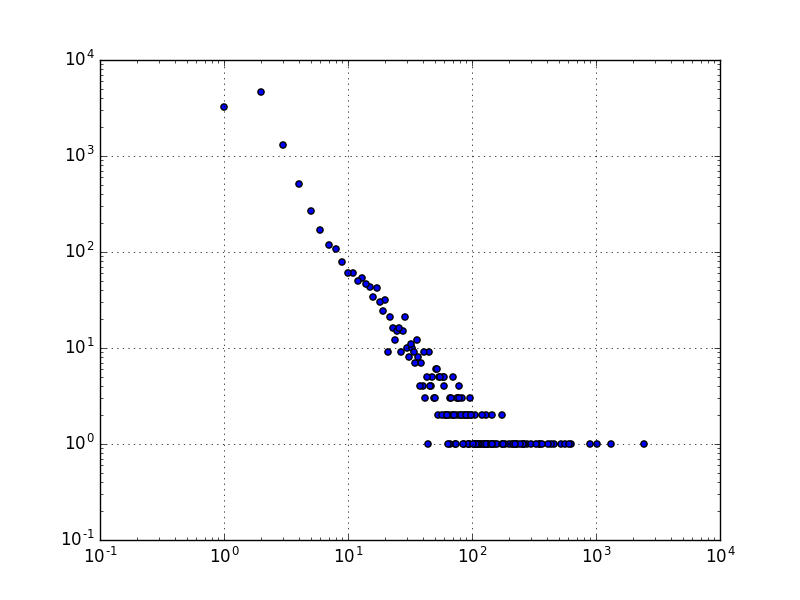
\includegraphics[width=\linewidth]{img/oregon-010519/degree_dist.png}
  \caption*{Oregon1-010519}
\endminipage\hfill
\minipage{0.33\textwidth}
  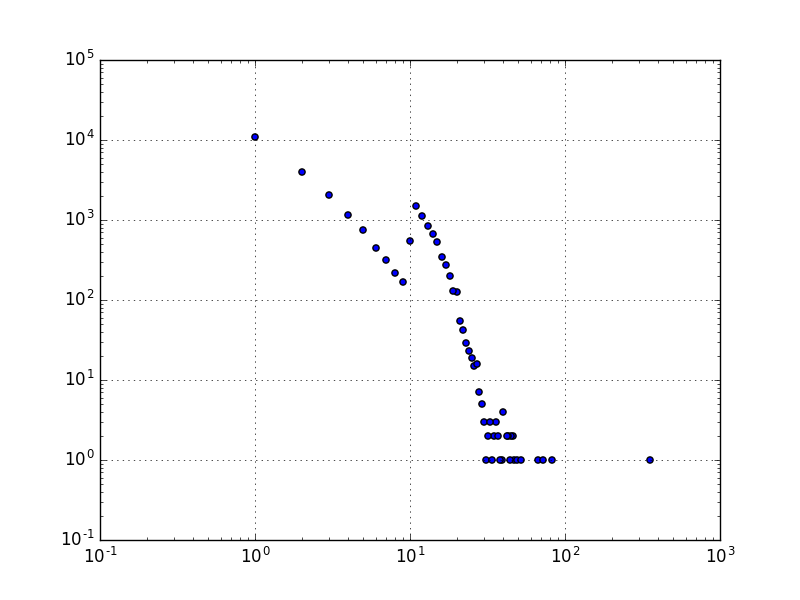
\includegraphics[width=\linewidth]{img/p2p-Gnutella24/degree_dist.png}
  \caption*{p2p-Gnutella24}
\endminipage\hfill
\minipage{0.33\textwidth}
  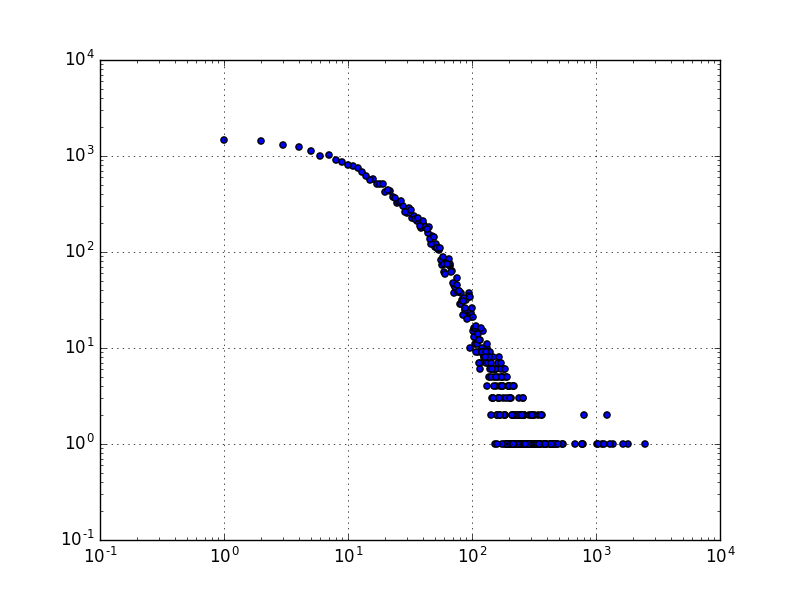
\includegraphics[width=\linewidth]{img/cit-HepTh/degree_dist.png}
  \caption*{cit-HepTh}
\endminipage
\end{figure}

Observations
\begin{itemize}
\item Most datasets exhibit a strong power law relation between degree and count. A large fraction of nodes (users) have very low degrees or very few connections. 
\item \textbf{P2P networks} (p2p-Gnutella24, pep-Gnutella25) exhibits a spike around degree = 10, implying that people tend to connect with 10 peers.
\item Some networks such as Facebook and \textbf{citation networks} do not follow a power law in degree range [1 - 10]. They look more like log-logistic. Taking Facebook for example, there are a lot of people with 1-10 friends, but the number of people with 1 friend and 10 friend does not differ much. Speaking in a formal way, nodes with a degree between 1 - 10 have similar counts.
\item We can also spot some outliers with only one connection in \{soc-Slashdot0811, soc-Slashdot0922\}, which probably means newly registered accounts in Slashdot Zoo, but they are less likely to get only one friend compared to the normal trend of other networks. Another outlier can be observed in dataset \{p2p-Gnutella 24\} where one node has a much higher degree = 200, probably because it functions as the central server in p2p network.
\end{itemize}

\subsubsection{Pagerank Distribution}

CCDF\quad x-axis: pagerank score \quad y-axis: count($\geq$ score)

\begin{figure}[H]
\minipage{0.33\textwidth}
  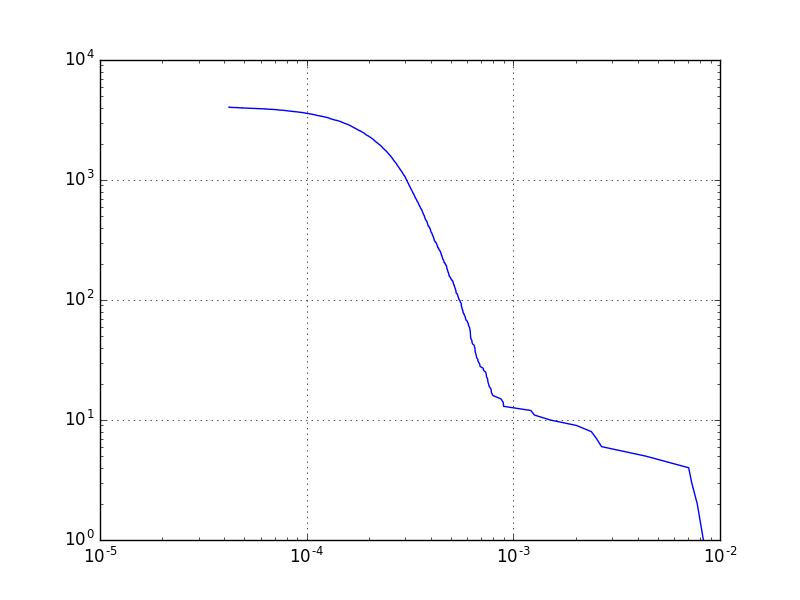
\includegraphics[width=\linewidth]{img/facebook/pagerank_ccdf.png}
  \caption*{Facebook}
\endminipage\hfill
\minipage{0.33\textwidth}
  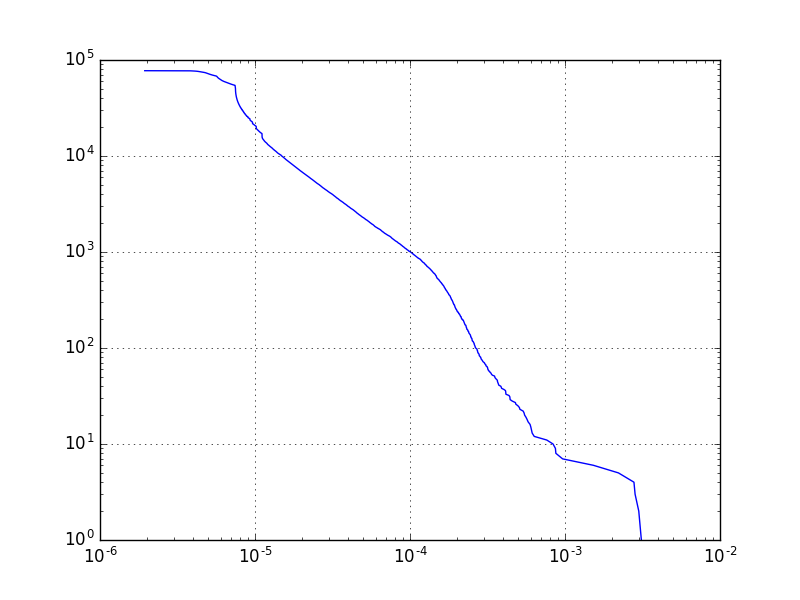
\includegraphics[width=\linewidth]{img/slashDot/pagerank_ccdf.png}
  \caption*{soc-Slashdot0811}
\endminipage\hfill
\minipage{0.33\textwidth}
  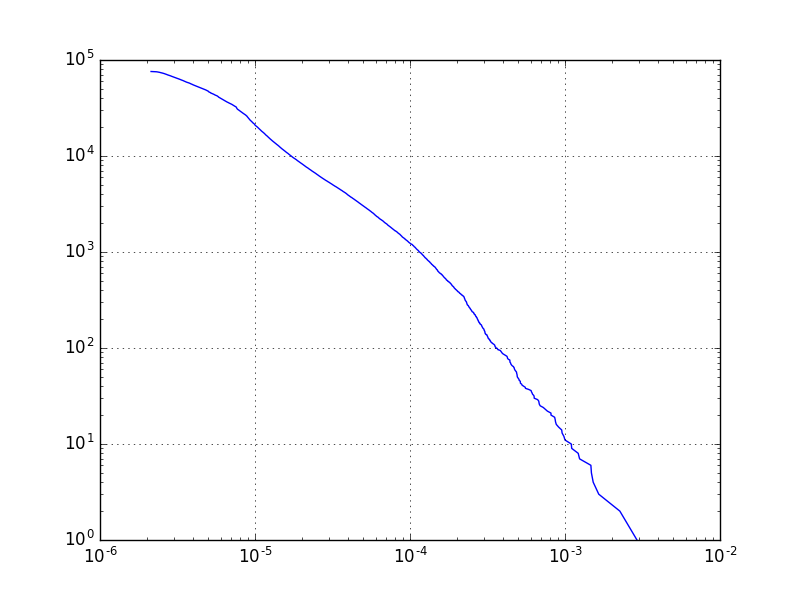
\includegraphics[width=\linewidth]{img/soc-E/pagerank_ccdf.png}
  \caption*{soc-Epinions1}
\endminipage
\end{figure}
\begin{figure}[H]
\minipage{0.33\textwidth}
  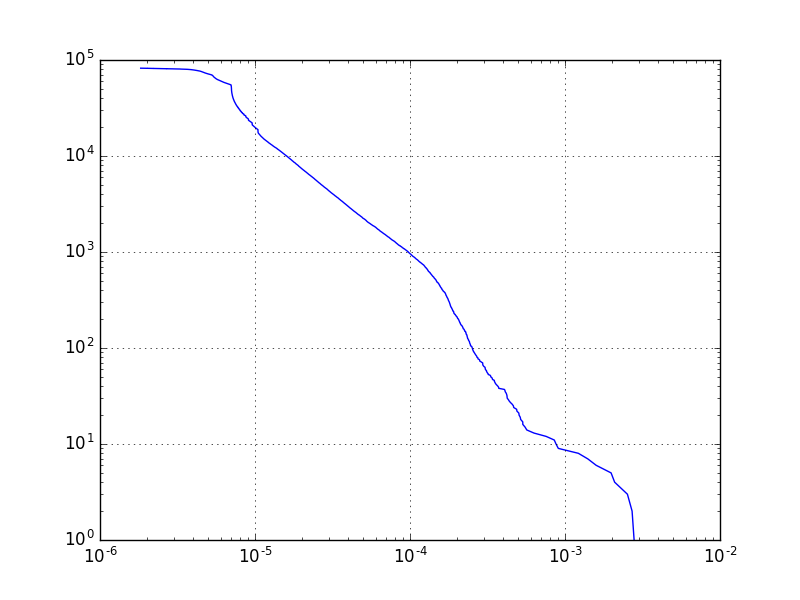
\includegraphics[width=\linewidth]{img/slashDot09/pagerank_ccdf.png}
  \caption*{soc-Slashdot0922}
\endminipage\hfill
\minipage{0.33\textwidth}
  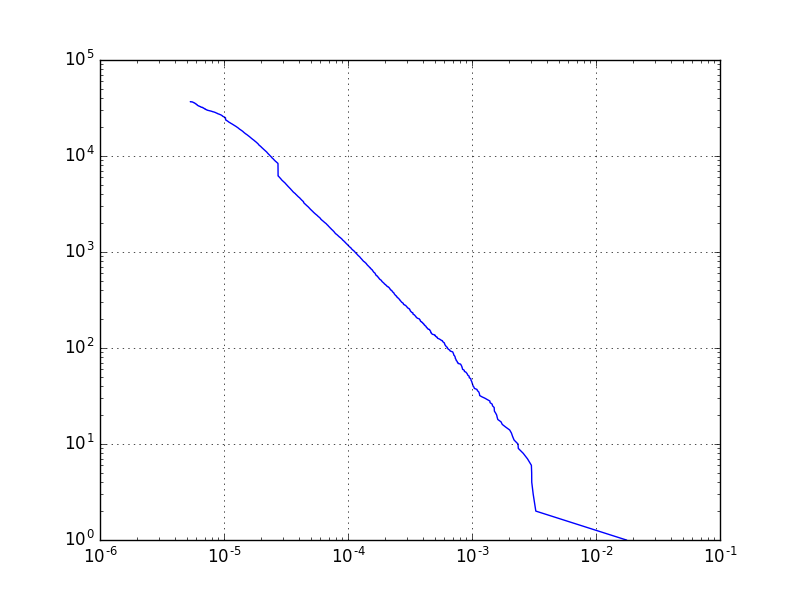
\includegraphics[width=\linewidth]{img/email/pagerank_ccdf.png}
  \caption*{email-Enron}
\endminipage\hfill
\minipage{0.33\textwidth}
  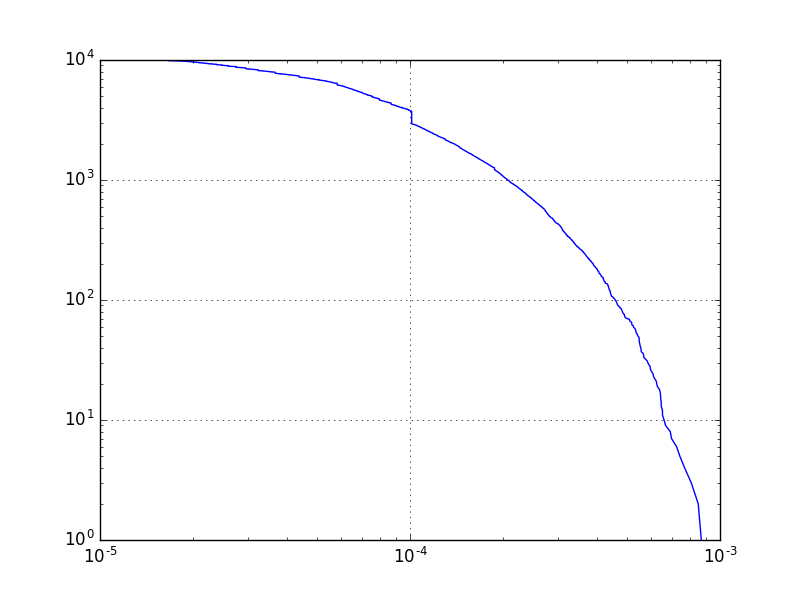
\includegraphics[width=\linewidth]{img/ca-HepTh/pagerank_ccdf.png}
  \caption*{ca-HepTh}
\endminipage
\end{figure}
\begin{figure}[H]
\minipage{0.33\textwidth}
  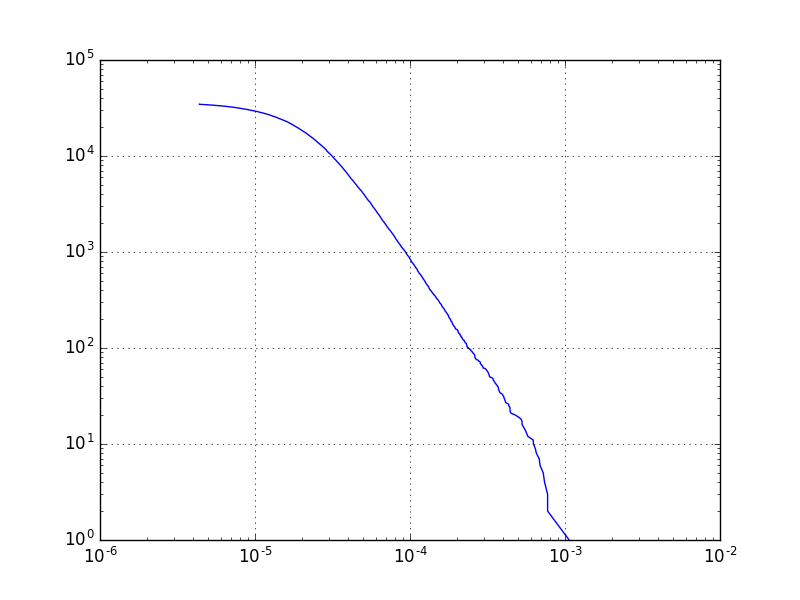
\includegraphics[width=\linewidth]{img/cit-HepPh/pagerank_ccdf.png}
  \caption*{cit-HepPh}
\endminipage\hfill
\minipage{0.33\textwidth}
  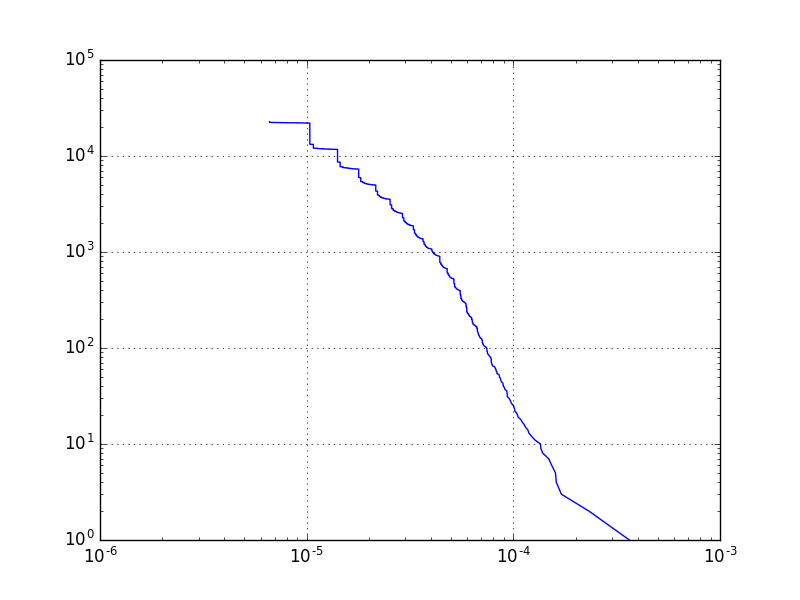
\includegraphics[width=\linewidth]{img/p2p-Gnutella25/pagerank_ccdf.png}
  \caption*{p2p-Gnutella25}
\endminipage\hfill
\minipage{0.33\textwidth}
  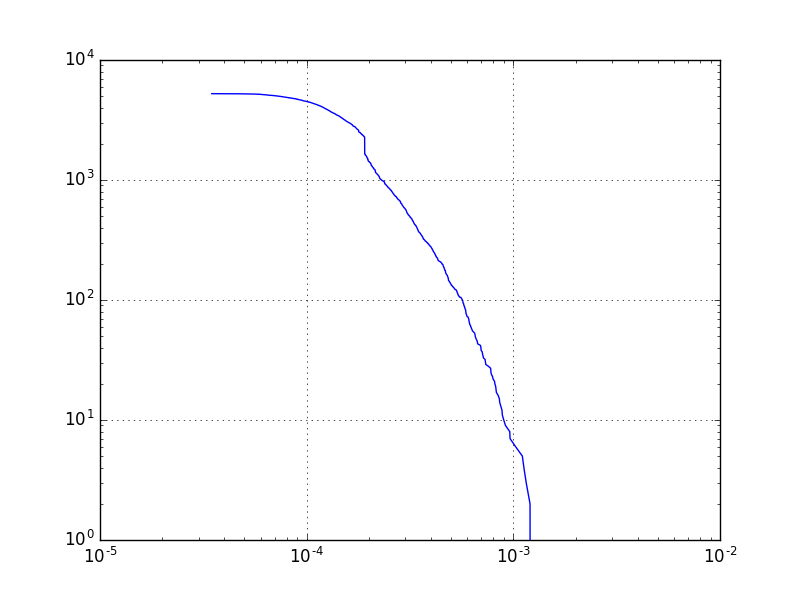
\includegraphics[width=\linewidth]{img/ca-GrQc/pagerank_ccdf.png}
  \caption*{ca-GrQc}
\endminipage
\end{figure}
\begin{figure}[H]
\minipage{0.33\textwidth}
  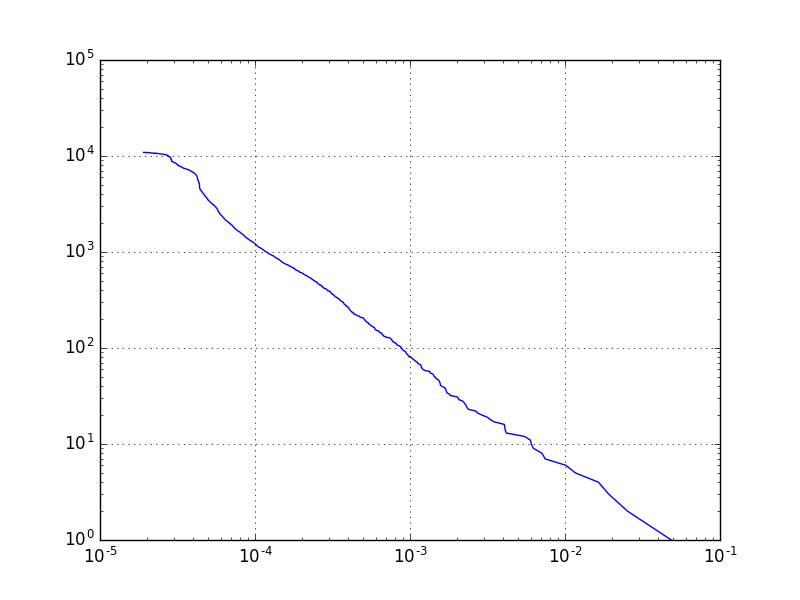
\includegraphics[width=\linewidth]{img/oregon-010331/pagerank_ccdf.png}
  \caption*{Oregon1-010331}
\endminipage\hfill
\minipage{0.33\textwidth}
  \includegraphics[width=\linewidth]{img/wiki-Vote/pagerank_ccdf.png}
  \caption*{wiki-Vote}
\endminipage\hfill
\minipage{0.33\textwidth}
  \includegraphics[width=\linewidth]{img/ca-Astro/pagerank_ccdf.png}
  \caption*{ca-Astro}
\endminipage
\end{figure}
\begin{figure}[H]
\minipage{0.33\textwidth}
  \includegraphics[width=\linewidth]{img/oregon-010519/pagerank_ccdf.png}
  \caption*{Oregon1-010519}
\endminipage\hfill
\minipage{0.33\textwidth}
  \includegraphics[width=\linewidth]{img/p2p-Gnutella24/pagerank_ccdf.png}
  \caption*{p2p-Gnutella24}
\endminipage\hfill
\minipage{0.33\textwidth}
  \includegraphics[width=\linewidth]{img/cit-HepTh/pagerank_ccdf.png}
  \caption*{cit-HepTh}
\endminipage
\end{figure}

Observations
\begin{itemize}
\item Via CCDF plots, we see many datasets follow power law between pagerank score and counts. This implies that only a few \texttt{'famous'} users own large impacts, while most \texttt{'ordinary'} users have small pagerank score $\sim [10^{-5}, 10^{-4}]$
\item However, for facebook dataset, the CCDF plot is not quite linear. This can be interpreted that a majority of Facebook users have low pagerank score and it is very hard to get pagerank score above a certain threshold.
\end{itemize}

\subsubsection{Eigen Value Distribution}

Scatter plot\quad x-axis: rank \quad y-axis: abs(eigen value)

\begin{figure}[H]
\minipage{0.33\textwidth}
  \includegraphics[width=\linewidth]{img/facebook/eig.png}
  \caption*{Facebook}
\endminipage\hfill
\minipage{0.33\textwidth}
  \includegraphics[width=\linewidth]{img/slashDot/eig.png}
  \caption*{soc-Slashdot0811}
\endminipage\hfill
\minipage{0.33\textwidth}
  \includegraphics[width=\linewidth]{img/soc-E/eig.png}
  \caption*{soc-Epinions1}
\endminipage
\end{figure}
\begin{figure}[H]
\minipage{0.33\textwidth}
  \includegraphics[width=\linewidth]{img/slashDot09/eig.png}
  \caption*{soc-Slashdot0922}
\endminipage\hfill
\minipage{0.33\textwidth}
  \includegraphics[width=\linewidth]{img/email/eig.png}
  \caption*{email-Enron}
\endminipage\hfill
\minipage{0.33\textwidth}
  \includegraphics[width=\linewidth]{img/ca-HepTh/eig.png}
  \caption*{ca-HepTh}
\endminipage
\end{figure}
\begin{figure}[H]
\minipage{0.33\textwidth}
  \includegraphics[width=\linewidth]{img/cit-HepPh/eig.png}
  \caption*{cit-HepPh}
\endminipage\hfill
\minipage{0.33\textwidth}
  \includegraphics[width=\linewidth]{img/p2p-Gnutella25/eig.png}
  \caption*{p2p-Gnutella25}
\endminipage\hfill
\minipage{0.33\textwidth}
  \includegraphics[width=\linewidth]{img/ca-GrQc/eig.png}
  \caption*{ca-GrQc}
\endminipage
\end{figure}
\begin{figure}[H]
\minipage{0.33\textwidth}
  \includegraphics[width=\linewidth]{img/oregon-010331/eig.png}
  \caption*{Oregon1-010331}
\endminipage\hfill
\minipage{0.33\textwidth}
  \includegraphics[width=\linewidth]{img/wiki-Vote/eig.png}
  \caption*{wiki-Vote}
\endminipage\hfill
\minipage{0.33\textwidth}
  \includegraphics[width=\linewidth]{img/ca-Astro/eig.png}
  \caption*{ca-Astro}
\endminipage
\end{figure}
\begin{figure}[H]
\minipage{0.33\textwidth}
  \includegraphics[width=\linewidth]{img/oregon-010519/eig.png}
  \caption*{Oregon1-010519}
\endminipage\hfill
\minipage{0.33\textwidth}
  \includegraphics[width=\linewidth]{img/p2p-Gnutella24/eig.png}
  \caption*{p2p-Gnutella24}
\endminipage\hfill
\minipage{0.33\textwidth}
  \includegraphics[width=\linewidth]{img/cit-HepTh/eig.png}
  \caption*{cit-HepTh}
\endminipage
\end{figure}

Observations
\begin{itemize}
\item We draw the top 10 eigen values of each dataset. It can be seen that \texttt{\{eigen value $\lambda_i$ - rank $i$\}} follows power law for most datasets.
\item Eigen value drops dramatically at rank 8, rank 9 and rank 10. It takes much longer time to converge for the calculation of these eigen values and their values are $\sim [0.1, 1]$. This implies that we can actually compress many realworld datasets with top 8 eigen values and eigen vectors without losing much information.
\end{itemize}

\subsubsection{Connected-component-size distribution}

Scatter plot\quad x-axis: component size \quad y-axis: count

\begin{figure}[H]
\minipage{0.33\textwidth}
  \includegraphics[width=\linewidth]{img/facebook/comp_dist.png}
  \caption*{Facebook}
\endminipage\hfill
\minipage{0.33\textwidth}
  \includegraphics[width=\linewidth]{img/slashDot/comp_dist.png}
  \caption*{soc-Slashdot0811}
\endminipage\hfill
\minipage{0.33\textwidth}
  \includegraphics[width=\linewidth]{img/soc-E/comp_dist.png}
  \caption*{soc-Epinions1}
\endminipage
\end{figure}
\begin{figure}[H]
\minipage{0.33\textwidth}
  \includegraphics[width=\linewidth]{img/slashDot09/comp_dist.png}
  \caption*{soc-Slashdot0922}
\endminipage\hfill
\minipage{0.33\textwidth}
  \includegraphics[width=\linewidth]{img/email/comp_dist.png}
  \caption*{email-Enron}
\endminipage\hfill
\minipage{0.33\textwidth}
  \includegraphics[width=\linewidth]{img/ca-HepTh/comp_dist.png}
  \caption*{ca-HepTh}
\endminipage
\end{figure}
\begin{figure}[H]
\minipage{0.33\textwidth}
  \includegraphics[width=\linewidth]{img/cit-HepPh/comp_dist.png}
  \caption*{cit-HepPh}
\endminipage\hfill
\minipage{0.33\textwidth}
  \includegraphics[width=\linewidth]{img/p2p-Gnutella25/comp_dist.png}
  \caption*{p2p-Gnutella25}
\endminipage\hfill
\minipage{0.33\textwidth}
  \includegraphics[width=\linewidth]{img/ca-GrQc/comp_dist.png}
  \caption*{ca-GrQc}
\endminipage
\end{figure}
\begin{figure}[H]
\minipage{0.33\textwidth}
  \includegraphics[width=\linewidth]{img/oregon-010331/comp_dist.png}
  \caption*{Oregon1-010331}
\endminipage\hfill
\minipage{0.33\textwidth}
  \includegraphics[width=\linewidth]{img/wiki-Vote/comp_dist.png}
  \caption*{wiki-Vote}
\endminipage\hfill
\minipage{0.33\textwidth}
  \includegraphics[width=\linewidth]{img/ca-Astro/comp_dist.png}
  \caption*{ca-Astro}
\endminipage
\end{figure}
\begin{figure}[H]
\minipage{0.33\textwidth}
  \includegraphics[width=\linewidth]{img/oregon-010519/comp_dist.png}
  \caption*{Oregon1-010519}
\endminipage\hfill
\minipage{0.33\textwidth}
  \includegraphics[width=\linewidth]{img/p2p-Gnutella24/comp_dist.png}
  \caption*{p2p-Gnutella24}
\endminipage\hfill
\minipage{0.33\textwidth}
  \includegraphics[width=\linewidth]{img/cit-HepTh/comp_dist.png}
  \caption*{cit-HepTh}
\endminipage
\end{figure}

Observations
\begin{itemize}
\item \textbf{Social networks} (Facebook, soc-Slashdot, soc-Epinions), \textbf{P2P networks} (p2p-Gnutella) and \textbf{Autonomous networks} (Oregon1) are very well and fully connected, resulting in only one or two connected components.
\item Other networks such as \textbf{Collaboration networks} and \textbf{Citation networks} exhibits a power law relation for components of small \& medium sizes. For these networks, there exists one large component whose size is greater than sum of the rest. 
\end{itemize}


\subsubsection{Coreness Value Distribution}

Scatter plot\quad x-axis: k-core value \quad y-axis: count

\begin{figure}[H]
\minipage{0.33\textwidth}
  \includegraphics[width=\linewidth]{img/facebook/kcore_dist.png}
  \caption*{Facebook}
\endminipage\hfill
\minipage{0.33\textwidth}
  \includegraphics[width=\linewidth]{img/slashDot/kcore_dist.png}
  \caption*{soc-Slashdot0811}
\endminipage\hfill
\minipage{0.33\textwidth}
  \includegraphics[width=\linewidth]{img/soc-E/kcore_dist.png}
  \caption*{soc-Epinions1}
\endminipage
\end{figure}
\begin{figure}[H]
\minipage{0.33\textwidth}
  \includegraphics[width=\linewidth]{img/slashDot09/kcore_dist.png}
  \caption*{soc-Slashdot0922}
\endminipage\hfill
\minipage{0.33\textwidth}
  \includegraphics[width=\linewidth]{img/email/kcore_dist.png}
  \caption*{email-Enron}
\endminipage\hfill
\minipage{0.33\textwidth}
  \includegraphics[width=\linewidth]{img/ca-HepTh/kcore_dist.png}
  \caption*{ca-HepTh}
\endminipage
\end{figure}
\begin{figure}[H]
\minipage{0.33\textwidth}
  \includegraphics[width=\linewidth]{img/cit-HepPh/kcore_dist.png}
  \caption*{cit-HepPh}
\endminipage\hfill
\minipage{0.33\textwidth}
  \includegraphics[width=\linewidth]{img/p2p-Gnutella25/kcore_dist.png}
  \caption*{p2p-Gnutella25}
\endminipage\hfill
\minipage{0.33\textwidth}
  \includegraphics[width=\linewidth]{img/ca-GrQc/kcore_dist.png}
  \caption*{ca-GrQc}
\endminipage
\end{figure}
\begin{figure}[H]
\minipage{0.33\textwidth}
  \includegraphics[width=\linewidth]{img/oregon-010331/kcore_dist.png}
  \caption*{Oregon1-010331}
\endminipage\hfill
\minipage{0.33\textwidth}
  \includegraphics[width=\linewidth]{img/wiki-Vote/kcore_dist.png}
  \caption*{wiki-Vote}
\endminipage\hfill
\minipage{0.33\textwidth}
  \includegraphics[width=\linewidth]{img/ca-Astro/kcore_dist.png}
  \caption*{ca-Astro}
\endminipage
\end{figure}
\begin{figure}[H]
\minipage{0.33\textwidth}
  \includegraphics[width=\linewidth]{img/oregon-010519/kcore_dist.png}
  \caption*{Oregon1-010519}
\endminipage\hfill
\minipage{0.33\textwidth}
  \includegraphics[width=\linewidth]{img/p2p-Gnutella24/kcore_dist.png}
  \caption*{p2p-Gnutella24}
\endminipage\hfill
\minipage{0.33\textwidth}
  \includegraphics[width=\linewidth]{img/cit-HepTh/kcore_dist.png}
  \caption*{cit-HepTh}
\endminipage
\end{figure}

Observations
\begin{itemize}
\item Most datasets follow power law between \texttt{kcore value - count}.
\item It is easy to spot some outliers in dataset soc-Slashdot. soc-Slashdot graph has several dozen nodes whose k-core value are 1, loosely connected with other nodes.
\end{itemize}

\subsubsection{Radius Distribution}

PDF\quad x-axis: raidus \quad y-axis: count

\begin{figure}[H]
\minipage{0.33\textwidth}
  \includegraphics[width=\linewidth]{img/facebook/radius_dist.png}
  \caption*{Facebook}
\endminipage\hfill
\minipage{0.33\textwidth}
  \includegraphics[width=\linewidth]{img/slashDot/radius_dist.png}
  \caption*{soc-Slashdot0811}
\endminipage\hfill
\minipage{0.33\textwidth}
  \includegraphics[width=\linewidth]{img/soc-E/radius_dist.png}
  \caption*{soc-Epinions1}
\endminipage
\end{figure}
\begin{figure}[H]
\minipage{0.33\textwidth}
  \includegraphics[width=\linewidth]{img/slashDot09/radius_dist.png}
  \caption*{soc-Slashdot0922}
\endminipage\hfill
\minipage{0.33\textwidth}
  \includegraphics[width=\linewidth]{img/email/radius_dist.png}
  \caption*{email-Enron}
\endminipage\hfill
\minipage{0.33\textwidth}
  \includegraphics[width=\linewidth]{img/ca-HepTh/radius_dist.png}
  \caption*{ca-HepTh}
\endminipage
\end{figure}
\begin{figure}[H]
\minipage{0.33\textwidth}
  \includegraphics[width=\linewidth]{img/cit-HepPh/radius_dist.png}
  \caption*{cit-HepPh}
\endminipage\hfill
\minipage{0.33\textwidth}
  \includegraphics[width=\linewidth]{img/p2p-Gnutella25/radius_dist.png}
  \caption*{p2p-Gnutella25}
\endminipage\hfill
\minipage{0.33\textwidth}
  \includegraphics[width=\linewidth]{img/ca-GrQc/radius_dist.png}
  \caption*{ca-GrQc}
\endminipage
\end{figure}
\begin{figure}[H]
\minipage{0.33\textwidth}
  \includegraphics[width=\linewidth]{img/oregon-010331/radius_dist.png}
  \caption*{Oregon1-010331}
\endminipage\hfill
\minipage{0.33\textwidth}
  \includegraphics[width=\linewidth]{img/wiki-Vote/radius_dist.png}
  \caption*{wiki-Vote}
\endminipage\hfill
\minipage{0.33\textwidth}
  \includegraphics[width=\linewidth]{img/ca-Astro/radius_dist.png}
  \caption*{ca-Astro}
\endminipage
\end{figure}
\begin{figure}[H]
\minipage{0.33\textwidth}
  \includegraphics[width=\linewidth]{img/oregon-010519/radius_dist.png}
  \caption*{Oregon1-010519}
\endminipage\hfill
\minipage{0.33\textwidth}
  \includegraphics[width=\linewidth]{img/p2p-Gnutella24/radius_dist.png}
  \caption*{p2p-Gnutella24}
\endminipage\hfill
\minipage{0.33\textwidth}
  \includegraphics[width=\linewidth]{img/cit-HepTh/radius_dist.png}
  \caption*{cit-HepTh}
\endminipage
\end{figure}

Observations
\begin{itemize}
\item Realworld graphs have small diameters. Most nodes follow \textbf{six degree principle} (their effective radius are 5-7). 
\item We see that radius distribution (in PDF graph) is multimodal.
\end{itemize}

\subsubsection{Degree VS PageRank Distribution}

Scatter plot\quad a-axis: degree \quad y-axis: pagerank score

\begin{figure}[H]
\minipage{0.33\textwidth}
  \includegraphics[width=\linewidth]{img/facebook/degreeVSpagerank.png}
  \caption*{Facebook}
\endminipage\hfill
\minipage{0.33\textwidth}
  \includegraphics[width=\linewidth]{img/slashDot/degreeVSpagerank.png}
  \caption*{soc-Slashdot0811}
\endminipage\hfill
\minipage{0.33\textwidth}
  \includegraphics[width=\linewidth]{img/soc-E/degreeVSpagerank.png}
  \caption*{soc-Epinions1}
\endminipage
\end{figure}
\begin{figure}[H]
\minipage{0.33\textwidth}
  \includegraphics[width=\linewidth]{img/slashDot09/degreeVSpagerank.png}
  \caption*{soc-Slashdot0922}
\endminipage\hfill
\minipage{0.33\textwidth}
  \includegraphics[width=\linewidth]{img/email/degreeVSpagerank.png}
  \caption*{email-Enron}
\endminipage\hfill
\minipage{0.33\textwidth}
  \includegraphics[width=\linewidth]{img/ca-HepTh/degreeVSpagerank.png}
  \caption*{ca-HepTh}
\endminipage
\end{figure}
\begin{figure}[H]
\minipage{0.33\textwidth}
  \includegraphics[width=\linewidth]{img/cit-HepPh/degreeVSpagerank.png}
  \caption*{cit-HepPh}
\endminipage\hfill
\minipage{0.33\textwidth}
  \includegraphics[width=\linewidth]{img/p2p-Gnutella25/degreeVSpagerank.png}
  \caption*{p2p-Gnutella25}
\endminipage\hfill
\minipage{0.33\textwidth}
  \includegraphics[width=\linewidth]{img/ca-GrQc/degreeVSpagerank.png}
  \caption*{ca-GrQc}
\endminipage
\end{figure}
\begin{figure}[H]
\minipage{0.33\textwidth}
  \includegraphics[width=\linewidth]{img/oregon-010331/degreeVSpagerank.png}
  \caption*{Oregon1-010331}
\endminipage\hfill
\minipage{0.33\textwidth}
  \includegraphics[width=\linewidth]{img/wiki-Vote/degreeVSpagerank.png}
  \caption*{wiki-Vote}
\endminipage\hfill
\minipage{0.33\textwidth}
  \includegraphics[width=\linewidth]{img/ca-Astro/degreeVSpagerank.png}
  \caption*{ca-Astro}
\endminipage
\end{figure}
\begin{figure}[H]
\minipage{0.33\textwidth}
  \includegraphics[width=\linewidth]{img/oregon-010519/degreeVSpagerank.png}
  \caption*{Oregon1-010519}
\endminipage\hfill
\minipage{0.33\textwidth}
  \includegraphics[width=\linewidth]{img/p2p-Gnutella24/degreeVSpagerank.png}
  \caption*{p2p-Gnutella24}
\endminipage\hfill
\minipage{0.33\textwidth}
  \includegraphics[width=\linewidth]{img/cit-HepTh/degreeVSpagerank.png}
  \caption*{cit-HepTh}
\endminipage
\end{figure}

Observations
\begin{itemize}
\item In log-log scale, degree and pagerank score are positively correlated and approximately growing linearly.
\item \textbf{P2P networks} and \textbf{collaboration networks} are much more sparse and scattered compared to others. 
\item Some datasets e.g.\texttt{cit-HepPh}, we can observe that pagerank score grows super-linearly with degree. This means that growing connections can bring in even bigger impacts.
\end{itemize}

\subsubsection{Degree VS Coreness Distribution}

Scatter plot\quad x-axis: degree \quad y-axis: k-core value

\begin{figure}[H]
\minipage{0.33\textwidth}
  \includegraphics[width=\linewidth]{img/facebook/degreeVSkcore.png}
  \caption*{Facebook}
\endminipage\hfill
\minipage{0.33\textwidth}
  \includegraphics[width=\linewidth]{img/slashDot/degreeVSkcore.png}
  \caption*{soc-Slashdot0811}
\endminipage\hfill
\minipage{0.33\textwidth}
  \includegraphics[width=\linewidth]{img/soc-E/degreeVSkcore.png}
  \caption*{soc-Epinions1}
\endminipage
\end{figure}
\begin{figure}[H]
\minipage{0.33\textwidth}
  \includegraphics[width=\linewidth]{img/slashDot09/degreeVSkcore.png}
  \caption*{soc-Slashdot0922}
\endminipage\hfill
\minipage{0.33\textwidth}
  \includegraphics[width=\linewidth]{img/email/degreeVSkcore.png}
  \caption*{email-Enron}
\endminipage\hfill
\minipage{0.33\textwidth}
  \includegraphics[width=\linewidth]{img/ca-HepTh/degreeVSkcore.png}
  \caption*{ca-HepTh}
\endminipage
\end{figure}
\begin{figure}[H]
\minipage{0.33\textwidth}
  \includegraphics[width=\linewidth]{img/cit-HepPh/degreeVSkcore.png}
  \caption*{cit-HepPh}
\endminipage\hfill
\minipage{0.33\textwidth}
  \includegraphics[width=\linewidth]{img/p2p-Gnutella25/degreeVSkcore.png}
  \caption*{p2p-Gnutella25}
\endminipage\hfill
\minipage{0.33\textwidth}
  \includegraphics[width=\linewidth]{img/ca-GrQc/degreeVSkcore.png}
  \caption*{ca-GrQc}
\endminipage
\end{figure}
\begin{figure}[H]
\minipage{0.33\textwidth}
  \includegraphics[width=\linewidth]{img/oregon-010331/degreeVSkcore.png}
  \caption*{Oregon1-010331}
\endminipage\hfill
\minipage{0.33\textwidth}
  \includegraphics[width=\linewidth]{img/wiki-Vote/degreeVSkcore.png}
  \caption*{wiki-Vote}
\endminipage\hfill
\minipage{0.33\textwidth}
  \includegraphics[width=\linewidth]{img/ca-Astro/degreeVSkcore.png}
  \caption*{ca-Astro}
\endminipage
\end{figure}
\begin{figure}[H]
\minipage{0.33\textwidth}
  \includegraphics[width=\linewidth]{img/oregon-010519/degreeVSkcore.png}
  \caption*{Oregon1-010519}
\endminipage\hfill
\minipage{0.33\textwidth}
  \includegraphics[width=\linewidth]{img/p2p-Gnutella24/degreeVSkcore.png}
  \caption*{p2p-Gnutella24}
\endminipage\hfill
\minipage{0.33\textwidth}
  \includegraphics[width=\linewidth]{img/cit-HepTh/degreeVSkcore.png}
  \caption*{cit-HepTh}
\endminipage
\end{figure}

Observations
\begin{itemize}
\item Like previous sections, degree VS coreness follows the same trend. Node's degree and kcore value are positively correlated and growing linearly. 
\item \textbf{P2P networks} and \textbf{collaboration networks} are not as dense as others. For such networks, kcore values and degree values are much more limited in a small range.
\end{itemize}

\subsection{Conclusions}

We have provided over 15 observations in the above sections. In general, we see find most graphs follow the power law either in scatter / PDF / CCDF form, i.e. a majority of nodes have low degrees / pagerank scores / k-core values. We also spotted some anomolies from plots. 

\section{Labor Division}

\begin{itemize}
\item Yuwei Zhang: Degree distribution, Eigen Value distribution, Radius Distribution, Degree VS PageRank Distribution
\item Silun Wang: Pagerank Distribution, Connected-component-size Distribution, Coreness Value Distribution, Degree VS Coreness Distribution
\end{itemize}

\section{Acknowledgement}

We would like to thank Nijith Jacob and Sharif Doghmi for their previous work on Graph Miner toolset. We also acknowledge SNAP for the dataset.



\bibliography{BIB/christosref,BIB/other}
\bibliographystyle{plain}


\end{document}
